\documentclass{article}

\usepackage[dblblindworkshop]{neurips_2026}
\workshoptitle{Personalized, Aligned, Long-Term Memory for AI Systems (PALM)}

\usepackage[utf8]{inputenc}
\usepackage[T1]{fontenc}
\usepackage{amsmath,amssymb}
\usepackage{booktabs}
\usepackage{multirow}
\usepackage{float}
\usepackage{graphicx}
\usepackage{microtype}

\usepackage[hidelinks]{hyperref}
\usepackage{url}

% Metadata scrub for the double-blind build.
\hypersetup{pdftitle={},pdfauthor={},pdfsubject={},pdfkeywords={},pdfcreator={},pdfproducer={}}

\title{Retention You Can Predict, Scope and Delete:\\ a $(\mu,\gamma,T)$ Law and a Structural Deletion Guarantee\\ for a Physics-Structured Memory Store}

% \author is unused: [dblblindworkshop] typesets "Anonymous Author(s)".

\begin{document}
\maketitle
\begin{abstract}
% [AND - The Setup/Context]
Existing memory systems enforce retention via explicit bookkeeping policies. Forgetting or deletion thereby relies on methods like decay factors, expiry timestamps, or learned forget gates, which dictate when a specific entry expires.
% [BUT - The Conflict/Gap]
However, these programmatic rules do not specify the physical rate of value degradation, the continuous dynamical effect of tuning retention parameters, or the exact residual state of the network following an item's removal.
% [THEREFORE - The Resolution/Action]
In this work, we resolve these ambiguities by formalizing forgetting as a dynamical property of a physics-structured memory store: specifically, one produced by a damped symplectic step of a learned Hamiltonian. Our retention policy is defined by a computable physical budget parameterized by three variables: the stored direction's spectral mass $\mu$, the damping $\gamma$, and the temperature $T$. We demonstrate three core properties of this architecture. First, the retention dial possesses a computable critical point: retention half-life is non-monotonic in friction, forming a V-curve minimized at $\gamma_{\rm crit}=2\varepsilon\mu$. This curve spans approximately 11 orders of magnitude in $\mu^2$ and holds across both designed and emergent (learned-MLP) units. Second, retention is rigorously scopeable: at $T>0$, friction preserves memory while temperature erases it. A localized friction hole thus acts as a memory vault, demonstrating a $107.77\pm4.78\times$ retention factor on designed architectures. Finally, removal is purely structural: under canonical \citet{blelloch_strongly_2007} placement, store-level deletion is exact. Post-deletion, the store is byte-identical to a state that never held the item, governed by defined operational conditions, on a designed, non-learned 3-dimensional datastore at capacities 8--64.
\end{abstract}

\section{Introduction}\label{sec:intro}

To contextualize the operational constraints of modern memory systems, we begin with deployed retention policies. Most deployed memory stores currently operate under retention/deletion mechanisms: a decay factor, an invalidation timestamp, a learned forget gate, or an explicit \texttt{DELETE} call. Despite these mechanisms, forgetting remains a critical failure mode that standard benchmarks often fail to adequately measure \citep{yang_control-plane_2026,uddin_recall_2026}. A programmatic policy is not a fundamental physical law. For instance, one cannot read the half-life of a stored value off a trained LSTM, identify the exact mechanism that tunes this half-life, or verify the latent mathematical residue once a value is removed.

This gap in fundamental understanding is widest at the point of data removal. Contemporary agent-memory research supplies robust mechanisms for writing, consolidating, and retrieving data. However, for deletion, the standard approach relies on superficial bookkeeping, such as a timestamp or a dropped row \citep{rasmussen_zep_2025,chhikara_mem0_2025}, which leaves measurable residue within the network architecture even after the entry is nominally deleted \citep{chakraborttii_ghost_2026,wang_memleak_2026}. Further related work is presented in App.~\ref{app:related}

In this work, we propose and analyze a memory framework where forgetting is a prescribed dynamical property of the store, governed by parameters that can be set, targeted, and analyzed in closed form, rather than an emergent side effect or an external bookkeeping rule. By modeling the store as a physical system, we provide computable answers to three core operational questions:
\begin{enumerate}
    \item What is the exact retention policy, and where does its critical point lie? (Sec.~\ref{sec:vcurve})
    \item Can retention be specifically scoped to a single localized item? (Sec.~\ref{sec:vault})
    \item Is structural deletion truly absolute, and what information mathematically leaks? (Sec.~\ref{sec:deletion})
\end{enumerate}

\paragraph{Methodological Foundations.}
The memory store is constructed as a physical system. The latent state $(q,p)$ (generated by some encoder) advances via a damped symplectic step of a learnable Hamiltonian, defined as $H=T(p)+V_\theta(q)$. The damping mechanism, defined as $p\mapsto(1-\gamma)p$, inherently supplies the forgetting function, while Langevin noise introduces the temperature $T$. Memory items can optionally be written as \emph{atoms}: localized energy wells superposed into a singular energy function that is subsequently read by dynamical relaxation. Our reference architecture is the Causal Learning Unit (CLU), first introduced as CHLU by \citet{jawahar_chlu_2026}. The core of this unit is exactly solvable: when diagonalized within the mass-whitened Hessian, a single damped step acts on each normal mode as a $2\times2$ matrix entirely fixed by $(\varepsilon\mu,\gamma)$. The spectral radius of this matrix dictates that specific mode's retention capacity.

\paragraph{Scope and Assumptions.}
To clarify the boundaries of our empirical claims, we define the following operational assumptions and constraints:
\begin{itemize}
    \item \textbf{Scale:} These early results rely on a novel, designed store. This is not a deployed, large-scale LLM agent memory, nor a generalized system benchmark.
    \item \textbf{Claim Classification:} We report a fundamental mechanism bounded by measured physical laws, not an end-to-end system performance result.
    \item \textbf{Nomenclature:} borrowing from and building on CHLU~\citep{jawahar_chlu_2026}
    \begin{itemize}
        \item \emph{Inertial mass ($M_i$):} The learned diagonal of the kinetic term, where larger values result in slower dynamics.
        \item \emph{Spectral mass ($\mu_k^2$):} Defined as $\lambda_k(M^{-1/2}\nabla^2V_\theta M^{-1/2})$, where larger values indicate shorter memory retention. Retention claims always utilize $\mu$.
        \item \emph{Stored direction:} A written value occupies a near-flat coset direction.
        \item \emph{Integration step ($\varepsilon$):} Fixed at $0.05$.
    \end{itemize}
    \item \textbf{Evaluation Metrics:} Half-lives ($n_{1/2}$) are presented with their corresponding read tolerances ($\Delta$) and the thermal persistence length ($\ell_\theta=\varepsilon\sqrt{T/M}/(\gamma r_*)$, the coset register's physical resolution limit at temperature $T$).
    \item \textbf{Thermodynamic Consistency:} $T>0$ strictly requires the fluctuation--dissipation-consistent noise scale $\sigma^\star_i=\sqrt{M_iT\gamma(2-\gamma)}$ utilized alongside a Newtonian kinetic mode.
\end{itemize}

\section{Results}\label{sec:results}

\subsection{The Retention Dial Possesses a Computable Critical Point}\label{sec:vcurve}

Friction is not a monotone retention knob and the dial has a computable minimum. The turning point is fixed by the stored direction's spectral mass, meaning the optimal setting can be analytically predicted rather than empirically tuned. To understand the macro-dynamics of memory decay, we analyze damping as that retention dial.

The integration step is defined as conformally symplectic ($\det J=(1-\gamma)^d$) and scales to $(1-\gamma\phi(q'))^d$ when position-gated (this is derived in App.~\ref{app:deriv:2}, and the closed forms below in App.~\ref{app:derivation}). Our evaluation utilizes checkpoints comprising a dimension of 4, a hidden size of 64, $\varepsilon=0.05$, spanning 150 epochs. We assess both \textbf{designed units} (featuring an $SO(2)$-invariant $V_\theta$, across 5 seeds) and \textbf{emergent units} (utilizing an MLP $V_\theta$ trained on identical symmetric data, across 3 seeds).

The latch, the overdamped register, and the underdamped working memory are three specific operational regimes of a unified curve evaluated at two disparate values of $\mu$. On a fully trained, designed $SO(2)$ vacuum, the massive radial mode's retention half-life $n_{1/2}(\gamma)$ forms a V-curve, minimized at $\gamma_{\rm crit}=2\varepsilon\mu_{\rm rad}$ (Fig.~\ref{fig:massiveflat}, App.~\ref{app:budget}). The overdamped branch tracks the $\mu^{-2}$ law until $\varepsilon\mu\approx\gamma/2$, after which it saturates at a mass-independent floor. This yields log-slopes of $-1.006$ and between $+1.23$ and $+1.27$ across the 5 validation seeds (See App.~\ref{app:budget} for results). The flat coset (characterized by a Hessian $\mu^2\approx10^{-15}$) maps to the exact same curve at the limit $\mu\to0$, where $\gamma_{\rm crit}\to0$.

This fundamental law transfers directly to emergent units. Evaluating three emergent MLP checkpoints, the coset-tracked $T=0$ retention half-life: read on the near-flat stored direction that holds a written value, not on the stiff radial mode of the previous paragraph, though one law governs both. (Fig.~\ref{fig:collapse}) traces the identical V-curve framework: an argmin in units of $\gamma_{\rm crit}$, and respective log-slopes on the two asymptotic branches, across all 3 seeds (Figure~\ref{fig:lambdacoset}), with the measured values in Table~\ref{tab:numbers}. Spanning both architecture families, this curve holds consistently across a $\mu^2$ span of eleven orders (Table~\ref{tab:numbers}, Fig.~\ref{fig:collapse}). The low endpoint of that span is the ring-profile probe's resolution on a checkpoint whose Hessian $\mu^2$ is machine zero rather than a spectral mass, so eleven orders is one curve on one instrument (probe-floor tick marked in Fig.~\ref{fig:collapse-full}). In essence, the curve a designed unit follows is the curve a learned one follows, read at a different spectral mass.

\begin{figure}[htbp]
  \centering
  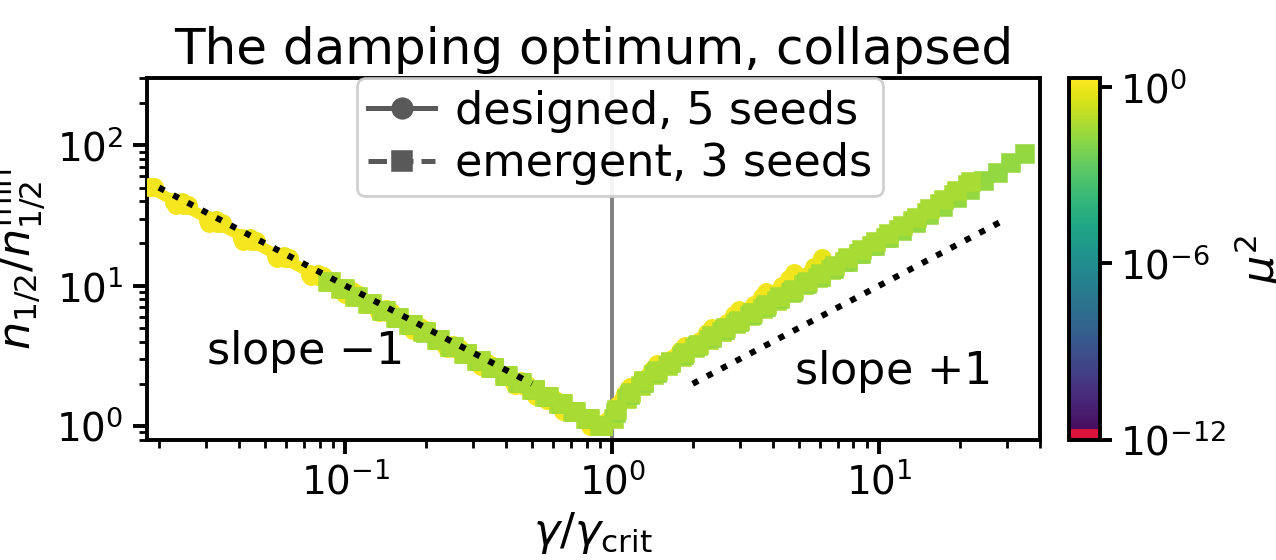
\includegraphics[width=0.6\linewidth]{figs/fig1_damping_optimum.png}
  \caption{\emph{The retention dial and its critical point, collapsed (headline).} Eight measured curves collapse onto one: five designed radial modes (circles, verification, $\mu^2_{\rm rad}=0.670$--$1.348$) and three emergent learned-MLP coset modes (squares, evidence, $\mu^2_{\rm soft}=2.0$--$5.4\times10^{-2}$, 3/3 seeds), against the $\mp1$ asymptotes; the designed flat coset is the $\mu\to0$ corner of the same curve. \emph{(One-step Jacobian; dim 4, hidden 64, $\varepsilon=0.05$, single-CPU; \texttt{langevin\_noise="fdt"}, Newtonian kinetic mode.)}}
  \label{fig:collapse}
\end{figure}

\textbf{Cross-Instrument Verification.} Because the primary measurements rely on one-step Jacobians, we re-measured the entire curve utilizing direct nonlinear rollout, extracting $n_{1/2}$ directly from the decay envelope's structural rate. The underlying shape is reproduced well on this second instrument (see Fig.~\ref{fig:twoinstruments}), the two argmins agreeing to $0.35\%$ in units of $\gamma_{\rm crit}$ (both readings in Table~\ref{tab:numbers}). This establishes that the gap between instruments dictates the level, not the fundamental law (see App.~\ref{app:emergent}).

\subsection{Scoping Retention: Friction Preserves, Temperature Erases}\label{sec:vault}

At the macro level, isolating a retention policy to a singular entry requires manipulating the physical dial locally. At absolute zero ($T=0$), a designed coset latches indefinitely across every friction setting we evaluated (Fig~\ref{fig:massiveflat}b; drift bound and $\gamma$ range in Table~\ref{tab:numbers}). Conversely, at $T>0$, the coset degrades via diffusion, and introducing friction decelerates this decay.

We establish that the diffusion coefficient of the stored coordinate is modeled as $D_\theta=\varepsilon T(2-\gamma)/(2F^2\gamma)$, where the coset scale $F^2=M r_*^2$ is the mass-weighted squared displacement of the latent state per unit stored coordinate (App.~\ref{app:deriv:6}), which we verified over a grid of $(\gamma,T)$ cells on the designed testbed (Table~\ref{tab:numbers}). Consequently, $n_{1/2}\propto\gamma^{+1}$. This sign flip ($\partial n_{1/2}/\partial\gamma>0$) holds universally across all evaluated seed and temperature combinations (Figure~\ref{fig:signflip}; diffusion-law diagnostics in Figure~\ref{fig:dlaw}, Appendix~\ref{app:budget}). Only temperature exhibits an inverse erasure effect ($\partial n_{1/2}/\partial T<0$).

\textbf{The Memory Vault Mechanism.} We propose the memory vault: a position-gated friction field that is absorb-only. A localized spatial hole within this field acts simultaneously as a brake, increasing dissipation, and a refrigerator, reducing the local effective temperature. This mechanism generates a retention vault factor of $(\gamma_{\rm eff}/\gamma)^2$ on designed architecture (Fig.~\ref{fig:vault}), read from the $\hat D_\theta$ estimator and quoted against a uniform-scalar-friction control at matched $\gamma_{\rm eff}$; the direct first-passage reading is boundary-layer biased on the outside arm ($\ell_\theta/\Delta=0.079$) and is therefore not the quoted vault. All four readings (the $\hat D_\theta$ vault, the scalar control, the first-passage value, and the local temperature) are in Table~\ref{tab:numbers}. Crucially, this localized field mathematically confines the register: the state fraction outside the boundary ($|\theta|>1$ rad) drops definitively to $0$ within the hole (see Fig.~\ref{fig:vault-emergent} and App.~\ref{app:vault}). Effectively, the vault factor is how much longer a written value is retained inside the hole than outside it.

\begin{figure}[htbp]\centering
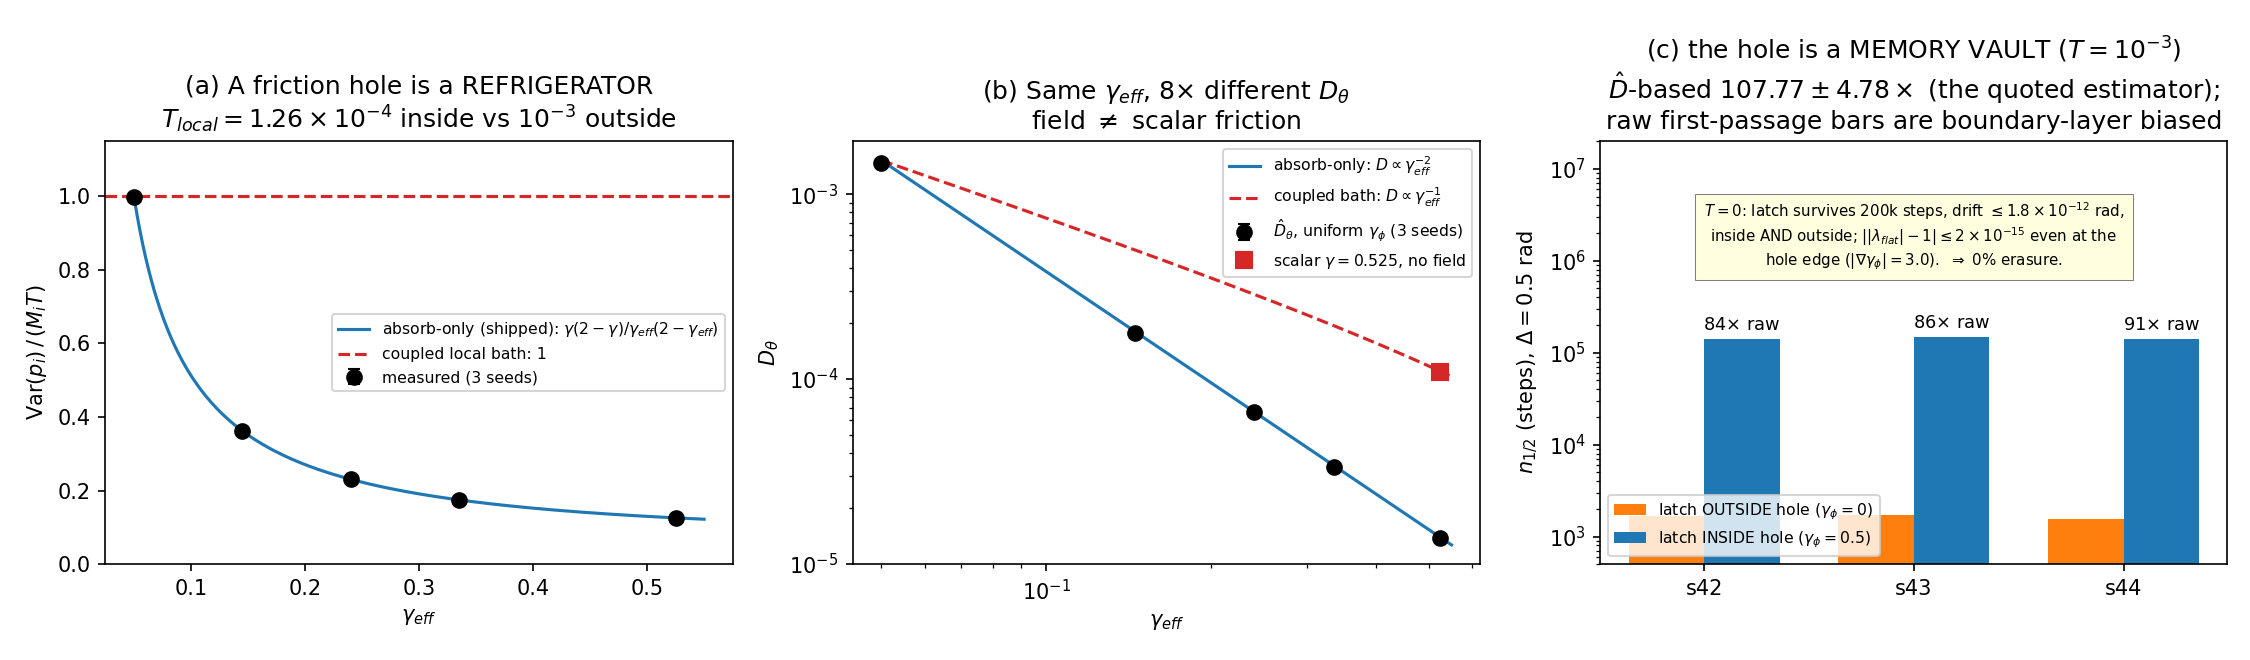
\includegraphics[width=\linewidth]{figs/fig2_vault.png}
\caption{The friction hole as a memory vault, on the designed arm. (a) The hole is a refrigerator: the momentum variance follows the absorb-only curve and rejects the coupled-bath prediction, giving $T_{\rm local}=1.26\times10^{-4}$ inside against $10^{-3}$ outside. (b) At the same $\gamma_{\rm eff}$ the diffusion constant differs by $8\times$ between a friction field and a scalar friction, which is the mechanism statement in one panel. (c) The vault factor: $107.77\pm4.78\times$ from the $\hat D_\theta$ estimator; the per-seed bars beneath it are raw first-passage ratios, boundary-layer biased on the outside arm, which is why the pooled first-passage reading of $86.97\pm2.94\times$ is not quoted as the vault. The inset states the $T=0$ control: the hole erases nothing. \emph{Designed $SO(2)$ with an analytic field, 3 seeds, $T=10^{-3}$, $\Delta=0.5$ rad, \texttt{langevin\_noise="fdt"}, Newtonian kinetic mode, single-CPU: verification.}}
\label{fig:vault}
\end{figure}

\subsection{Structural Deletion: Absolute Guarantees, Lifetime Trade-offs, and Residual Leakage}\label{sec:deletion}

In standard architectures, deleting an item from memory relies on stochastic, best-effort heuristics, such as dropping active rows or writing system tombstones. We evaluate whether the store's intrinsic physical state can be reduced to a pure function of its live set alone, i.e., whether the layout depends only on which items are currently stored, not on the order or history of the writes that stored them. When data points are continuously superposed into a singular energy function, standard placement becomes inherently path-dependent.

To resolve this, we map memory placement canonically, ensuring it remains an exclusive function of the live records and the predefined geometry. Utilizing \citeauthor{blelloch_strongly_2007}'s \citeyearpar{blelloch_strongly_2007} stable-matching table rules, we establish exact store-level deletion. Our measurements (see App.~\ref{app:deletion}) confirm that with the waitlist engaged, store-level deletion remains exact across all evaluated loads ($0.29\times$ to $1.71\times$ of standard lattice capacity). Under explicit conditions (a budget sufficient for the cell count, zero baseline leakage, and priority/attribute-based eviction; recency-based eviction remains intrinsically history-dependent and is excluded), the physical layout of the store remains byte-identical to a temporal state that theoretically never encountered the deleted item. This is a store-level guarantee only; the frozen encoder and any residue of past writes in a learned landscape are separate channels, and we claim no certified $(\varepsilon,\delta)$ unlearning.

\paragraph{The Lifetime Trilemma and Residual Leakage:} Memory lifetimes are governed by a strict trilemma: exact value fidelity, amplitude-independent address hold, and amplitude-independent read latency. A system may only optimize two. We also note that physical decay provides architectural retrieval geometry rather than cryptographic privacy (App.~\ref{app:deletion}).


\section{Limitations and Future Work}\label{sec:limits}

To define the scope and bounds of our empirical evidence, we identify the following limitations and subsequent future pathways:
\begin{itemize}
    \item \textbf{Scale and Architecture Scope:} This extended abstract is strictly constrained to physics-structured memory stores (e.g. CLU). Early experiments are performed at dimension of 4, a hidden size of 64, and small-scale execution on a single CPU across 5 designed and 3 emergent seeds. No larger-scale performance is inferred and scaling is left to future work.
    \item \textbf{The Designed-Symmetry Precondition:} The exact $T=0$ retention latch currently requires precise continuous coset geometries that must be designed into the architecture.
    \item \textbf{Mandatory Thermodynamic Scope:} The raw $T/\gamma$-exponents cannot distinguish between designed and emergent units. Evaluating any state where $T>0$ requires the strict combination of \texttt{fdt} noise and Newtonian kinetic modes.
    \item \textbf{Deletion Scope:} The exact deletion guarantee applies strictly at the isolated store-level beneath set-function eviction models. Furthermore, recency-based eviction intrinsically breaks latent history independence and is thus excluded.
    \item \textbf{No Task-Level Results:} This work presents a theoretical concept with empirical validation. Testing on specific task-level benchmarks is left to future work.
    \item \textbf{Future Work Directions:} We intend to evaluate wider emergent collapses in $\mu^2$, remeasure the memory vault contrast, formally assess the amortized per-delete execution cost against flat datastore architectures, and construct localized temperature fields. Developing these to a practically feasible  and performant state at the scales required will allow end-to-end CLU-like Physics-structured units acting on real data to be able to re-organize a learned latent space in both a useful and controllable way
\end{itemize}

\bibliographystyle{plainnat}
\bibliography{refs}
% The reference below is retained verbatim from the hand-built list per task v5-cite-pass 2b.4:
% no refs.bib entry exists for it (no DOI; arXiv record unretrievable), so it cannot be cited by key.
\begin{itemize}
\item Jude, J., Perich, M. G., Miller, L. E., \& Hennig, M. H. (2023). Capturing cross-session neural population variability through self-supervised identification of consistent neuron ensembles. \emph{PMLR} 197:234--257.
\end{itemize}

\appendix

\section{Values Quoted in the Main Text}\label{app:numbers}

Sec.~\ref{sec:results} states its results in words; the measured values behind them are collected here (Tab.~\ref{tab:numbers}), each beside the arm it was measured on and the rider it must be quoted with. \emph{Arm} names the class of the measurement: \textbf{verification} = a \emph{designed testbed} (an architecturally designed $SO(2)$ potential), \textbf{evidence} = a \emph{learned system} (an MLP $V_\theta$ trained on symmetric data). Every value is repeated from the section or appendix named beside it; none is new here.

\begin{table}[!htb]\centering\footnotesize
\setlength{\tabcolsep}{4pt}
\caption{The measured values behind Sec.~\ref{sec:results}, with the arm each was measured on and the rider each must travel with. \emph{Arm}: \emph{verification} = designed testbed; \emph{evidence} = learned system. All rows come from the checkpoints and grids of Sec.~\ref{sec:vcurve} and Apps.~\ref{app:budget}--\ref{app:vault} (dim 4, hidden 64, $\varepsilon=0.05$, single-CPU); every $T>0$ cell uses \texttt{langevin\_noise="fdt"} with a Newtonian kinetic mode.}
\label{tab:numbers}
\begin{tabular}{p{0.165\linewidth}p{0.15\linewidth}p{0.15\linewidth}p{0.075\linewidth}p{0.28\linewidth}}
\toprule
Result & Quantity & Value & Arm & Scope / rider\\
\midrule
\multirow{3}{\linewidth}{V-curve, emergent arm (Sec.~\ref{sec:vcurve}, App.~\ref{app:emergent})}
 & argmin, one-step Jacobian & $0.902\pm0.003\times\gamma_{\rm crit}$ & evidence & 3 emergent MLP seeds, $T=0$; a learned potential, not a designed one\\
 & log-slope, overdamped branch & $-1.0020\pm0.0003$ & evidence & same 3 emergent seeds\\
 & log-slope, underdamped branch & $+1.116\pm0.011$ & evidence & same 3 emergent seeds\\
\addlinespace
Collapse span (Sec.~\ref{sec:vcurve}) & $\mu^2$ range spanned by the one curve & $[1.7\times10^{-12},\,7\times10^{-2}]$ & both arms & Probe resolution: the low endpoint is the ring-profile probe's resolution on a checkpoint whose Hessian $\mu^2$ is machine zero (\emph{not} a measured spectral mass)\\
\addlinespace
\multirow{2}{\linewidth}{Cross-instrument check (App.~\ref{app:emergent})}
 & argmin, rollout envelope rate & $0.9001\pm0.0052\times\gamma_{\rm crit}$ & evidence & 3 emergent seeds, $\delta=0.05$ rad\\
 & argmin, one-step Jacobian & $0.9032\pm0.0027\times\gamma_{\rm crit}$ & evidence & same cells; the instrument gap is a level, not a rate\\
\addlinespace
$T=0$ latch (Sec.~\ref{sec:vault}, App.~\ref{app:budget}) & coset drift & $\le4.9\times10^{-12}$ rad / 200k steps & verifi\-cation & designed $SO(2)$ coset, every $\gamma\in[0.002,0.5]$; $T=0$ only\\
\addlinespace
Coset diffusion law (Sec.~\ref{sec:vault}, App.~\ref{app:budget}) & $\hat D_\theta/D_\theta^{\rm pred}$ & $1.0068\pm0.0219$ & verifi\-cation & 25 $(\gamma,T)$ cells on one trained designed checkpoint (seed 44), $\Delta=0.5$ rad\\
\addlinespace
\multirow{4}{\linewidth}{Friction-hole vault (Sec.~\ref{sec:vault}, App.~\ref{app:vault})}
 & $T_{\rm local}$ inside vs.\ outside & $1.26\times10^{-4}$ vs.\ $10^{-3}$ & verifi\-cation & designed arm, $\gamma=0.05$, $\gamma_\phi=0.5$; absorb-only field\\
 & vault factor, $\hat D_\theta$ estimator & $107.77\pm4.78\times$ & verifi\-cation & the quoted vault: Designed $SO(2)$, 3 seeds, $T=10^{-3}$, $\Delta=0.5$ rad\\
 & scalar-friction control & $13.28\pm0.12\times$ & verifi\-cation & uniform scalar friction at matched $\gamma_{\rm eff}$, same cells\\
 & raw first-passage ratio & $86.97\pm2.94\times$ & verifi\-cation & boundary-layer biased on the outside arm ($\ell_\theta/\Delta=0.079$); \emph{not} the quoted vault\\
\bottomrule
\end{tabular}
\end{table}

\section{Extended Related Work}\label{app:related}

\paragraph{Retention Policies in Deployed Memory Systems:}
Agent memories operate as external data stores that a model actively writes to, retrieves from, and dynamically edits (e.g., MemGPT, \citealp{packer_memgpt_2024}; Mem0, \citealp{chhikara_mem0_2025}). Alternatively, bounded compressive states exist internal to the network (e.g., Infini-attention, \citealp{munkhdalai_leave_2024}). The retention policies governing these systems rely on scores and gates. Examples include a $0.995$ recency decay factor in ranking heuristics \citep{park_generative_2023}, Ebbinghaus decay functions applied to memory strength \citep{zhong_memorybank_2023}, learned per-memory expiration spans \citep{sukhbaatar_not_2021}, and dynamic forget gates $\alpha_t$ optimized during test time \citep{behrouz_titans_2024}. While the learned gate in Titans \citep{behrouz_titans_2024} is structurally similar to the retention dial discussed in Sec.~\ref{sec:vcurve}, none of these prior works establish physical retention laws, state explicit half-lives, define read tolerances, or mathematically price the information loss.

\paragraph{Deletion Mechanisms: Deployed and Formal:}
Current deployment architectures handle deletion via invalidation. For example, Zep invalidates contradicted edges with timestamps while preserving the latent record \citep{rasmussen_zep_2025}, and Mem0 simply drops rows from its active context. Conversely, exact byte-identity is crucial for security, as soft-deleted vectors in graph ANN databases remain reconstructible from raw index files \citep{chakraborttii_ghost_2026}. Recent benchmarking highlights that real-world deployment failures are predominantly forgetting failures \citep{yang_control-plane_2026}, with outdated retention driving significant recommendation errors \citep{uddin_recall_2026}. Formally, \emph{certified} removal is \citeauthor{guo_certified_2023}'s \citeyearpar{guo_certified_2023} Sec.~2, Eq.~(1), an $\varepsilon$ condition with an unnumbered $(\varepsilon,\delta)$ relaxation immediately after; exact methods delete by isolation, with cost and capacity formalisms in place \citep{bourtoule_machine_2019,ginart_making_2019,sekhari_remember_2021}. We sit functionally between these approaches: we offer a store-level, bit-exact structural guarantee based on canonical geometric placement \citep{blelloch_strongly_2007}, rather than a stochastic system-level unlearning heuristic.

\paragraph{Physical and Learned Forgetting Laws:}
While learned recurrent models like LSTMs \citep{hochreiter_long_1997} lack stateable physical forgetting laws, biological and artificial representational drift has been observed to reorganize internal unit representations over time \citep{aitken_geometry_2022}. Our work differs by tracking a specific coset coordinate under strictly defined physical dynamics. In theoretical physics, dissipation transitions type-A Nambu--Goldstone modes from propagating to diffusive states \citep{minami_spontaneous_2018}. Furthermore, strictly equivariant flows possess Lyapunov neutral modes \citep{mo_symmetry-protected_2026} that provide kinematic protection, a gap complementary to our established physical budget ($\mu^2$).

\section{The effects of $(\mu,\gamma,T)$: The Diffusion Law and the Sign Flip}\label{app:budget}

To ensure complete rigor, all metrics detailed here derive from the designed $SO(2)$ testbed, providing strict verification. Furthermore, all $T>0$ cells mandate the explicit use of \texttt{langevin\_noise="fdt"} operating within a Newtonian kinetic mode. The legacy reference default structure fundamentally violates these thermodynamic laws. Every reported half-life $n_{1/2}$ is paired unconditionally with its specific read tolerance $\Delta=0.5$ rad and its ratio $\ell_\theta/\Delta$.

\paragraph{Diffusion Law Diagnostics (25 Cells):} We evaluate a discrete $5\gamma\times5T$ grid utilizing seed 44. The ratio $\hat D_\theta/D_\theta^{\rm pred}$ yields $1.0068\pm0.0219$, bounded between a minimum of $0.9644$ and a maximum of $1.0484$. The gradient $d\log D/d\log T$ records values of $+0.998,+0.997,+0.992,+1.010,+1.006$. Simultaneously, the gradient $d\log D/d\log\gamma$ evaluates to $-1.014,-0.980,-0.999,-1.001,-0.982$ following the mathematical isolation of the discrete $(2-\gamma)$ factor.

\paragraph{Sign Flip Verification:} We observe $d\log n_{1/2}/d\log\gamma=+0.9552\pm0.0422$ at a baseline temperature of $T=10^{-3}$ across all 5 testing seeds, presenting positively in all 10/10 examined conditions. The measured effect size for the transition $\gamma:0.05\to0.2$ results in a precise $3.77\pm0.23\times$ increase ($\ell_\theta/\Delta<0.05$; seed-specific values: $3.55,3.64,3.61,3.89,4.15$). The inverse thermal driver measures at $d\log n_{1/2}/d\log T=-0.956$ to $-0.979$ within the deep-diffusive operational bounds.

\paragraph{Designed $T=0$ Latch Properties:} Evaluating absolute zero, the metric $\big||\lambda_{\rm flat}|-1\big|\le1.7\times10^{-14}$ across 22 specific $\gamma$ values on 5 independent seeds. Consequently, the observed drift is restricted to $\le4.9\times10^{-12}$ rad per 200k integration steps across 30/30 evaluated cells. This strongly contrasts with the $\gamma=0$ baseline control, which incurs a massive $142.7$ rad drift over a significantly shorter 20k steps.

\paragraph{Designed V-Curve Minimization:} The optimal minimum argmin lies between $0.076$ and $0.096$, against the computationally predicted bounds of $0.082$--$0.116$ (utilizing per-seed specific values $\mu^2_{\rm rad}=0.670,0.771,1.190,1.093,1.348$). The resulting asymptotic log-slopes measure $-1.006$ and between $+1.23$ and $+1.27$, enforcing a mass-independent floor of exactly $27.03$ steps measured at $\gamma=0.05$.

\begin{table}[!htb]\centering\small
\caption{The $T>0$ face of the budget, all four entries continuously measured on the designated designed testbed.}
\begin{tabular}{p{0.19\linewidth}p{0.40\linewidth}p{0.31\linewidth}}
\toprule
Stored Direction & $\partial n_{1/2}/\partial\gamma$ (Increased Friction) & $\partial n_{1/2}/\partial T$ (Increased Heat)\\
\midrule
Coset / flat (designed) & $>0$, friction \emph{preserves} ($+0.955\pm0.042$; $3.77\times$ at $\gamma:0.05\to0.2$) & $<0$, temperature \emph{erases} ($-0.956$ to $-0.979$)\\
\addlinespace
Massive (underdamped) & $<0$, friction shortens (slope $-1.006$) & $\approx0$; $T$ sets only the fluctuation floor (max/min $\le1.013$)\\
\bottomrule
\end{tabular}
\end{table}

\begin{figure}[htbp]
  \centering
  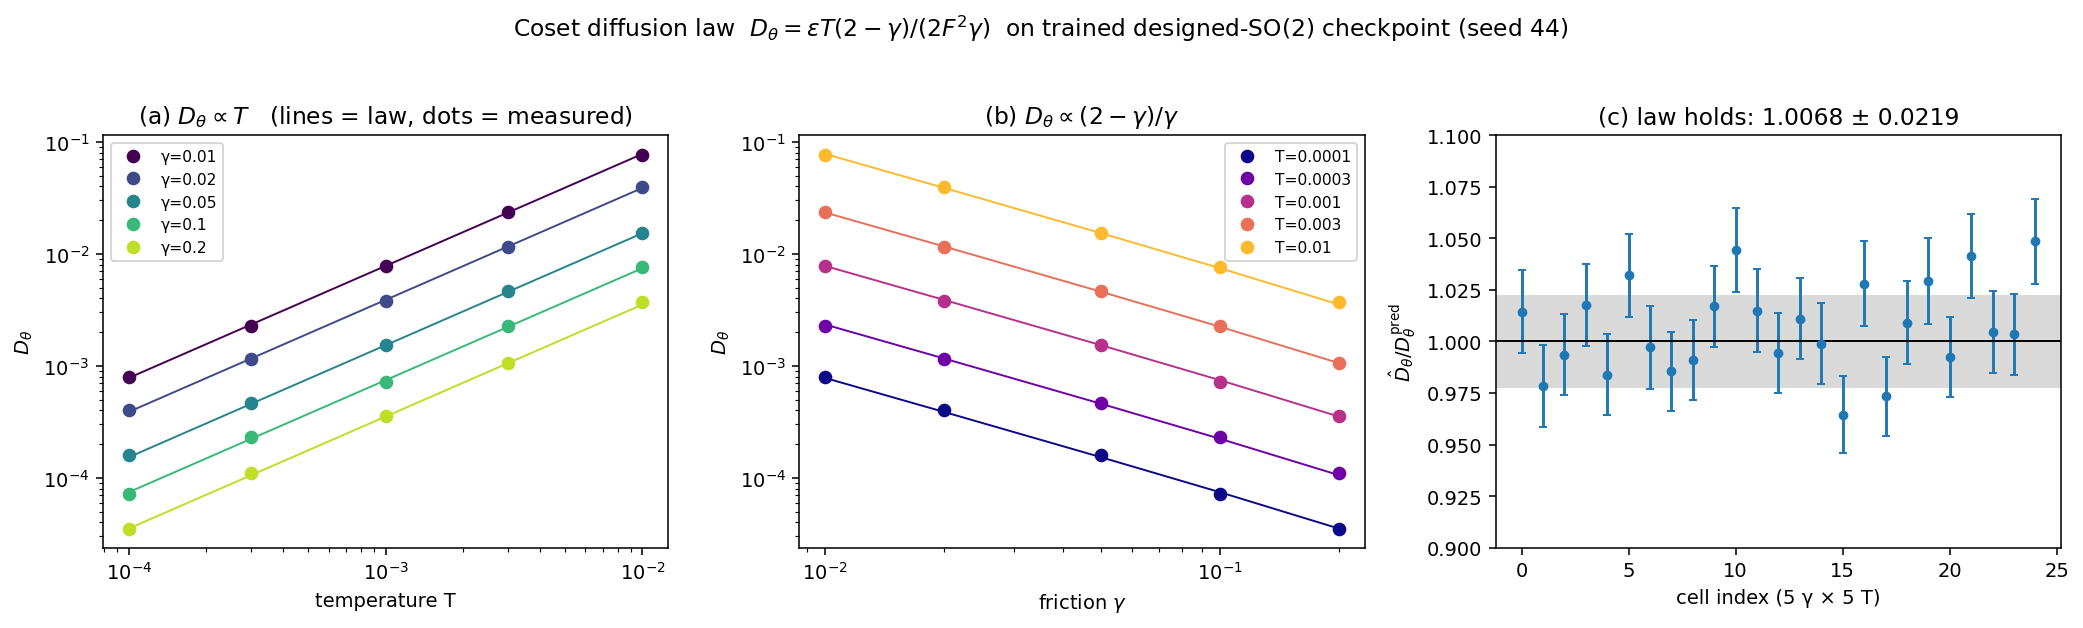
\includegraphics[width=\linewidth]{figs/figB_dlaw.png}
  \caption{The coset diffusion law, detailed systematically panel by panel. (a) $D_\theta\propto T$ measured precisely at five independent frictions; (b) $D_\theta\propto(2-\gamma)/\gamma$ evaluated at five specific temperatures; (c) the absolute ratio $\hat D_\theta/D_\theta^{\rm pred}$ compiled over all $25$ structural cells, reading exactly $1.0068\pm0.0219$ alongside the respective drawn band. \emph{Multi-seed status: evaluated utilizing one fully trained designed-$SO(2)$ checkpoint (seed 44).} \texttt{langevin\_noise="fdt"}, Newtonian kinetic mode, $\Delta=0.5$ rad. \emph{Designed testbed: validation of verification.}}
  \label{fig:dlaw}
\end{figure}

\begin{figure}[htbp]\centering
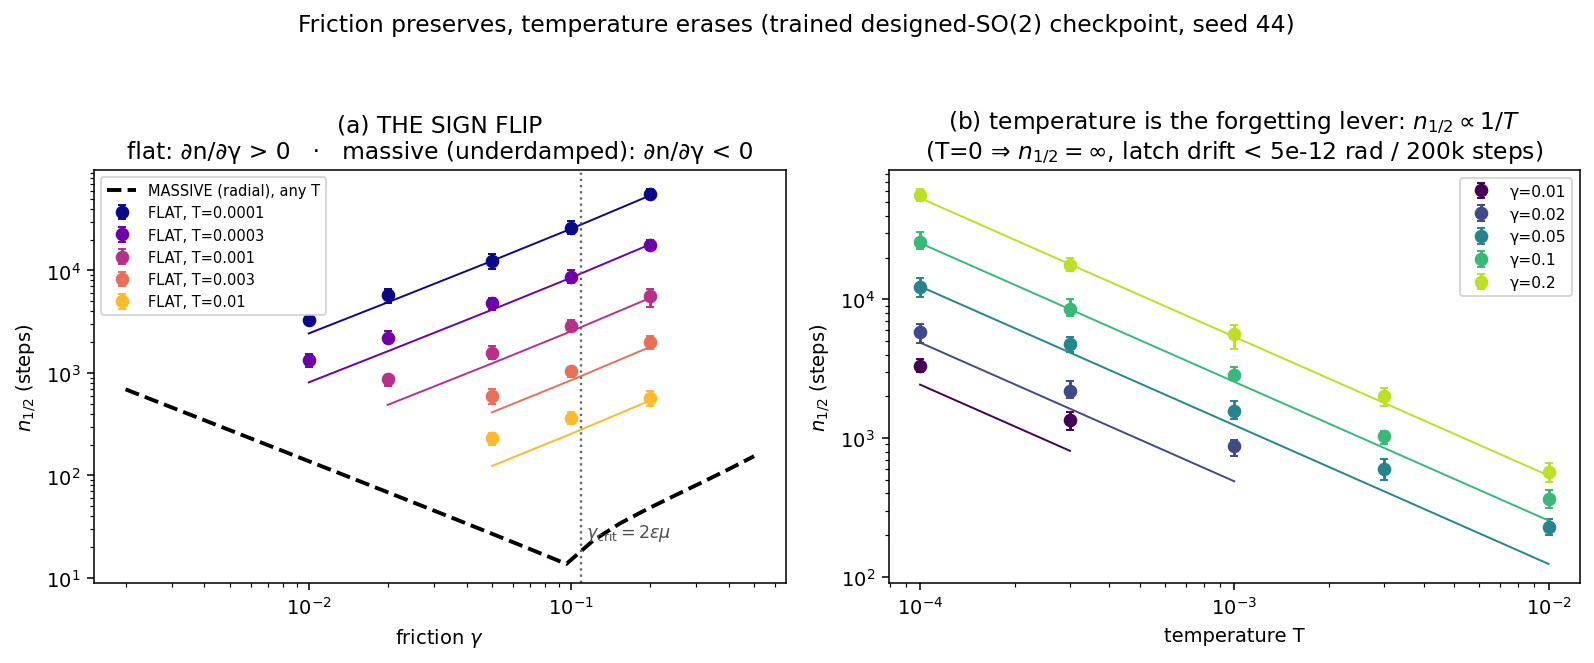
\includegraphics[width=\linewidth]{figs/figB_signflip.png}
\caption{The sign flip, and the lever that does erase. (a) The flat coset's half-life \emph{rises} with friction at every temperature, while the underdamped massive mode's falls --- the two stored directions respond to the dial with opposite sign, with $\gamma_{\rm crit}=2\varepsilon\mu$ marked. (b) Temperature is the forgetting lever, $n_{1/2}\propto1/T$ at every friction. \emph{Multi-seed status: one trained designed-$SO(2)$ checkpoint (seed 44); the $10/10$ seed $\times$ temperature statement and the $+0.9552\pm0.0422$ slope are this appendix's five-seed numbers, not this figure's.} \texttt{langevin\_noise="fdt"}, Newtonian kinetic mode, $\Delta=0.5$ rad. \emph{Designed testbed: verification.}}
\label{fig:signflip}
\end{figure}

\begin{figure}[htbp]\centering
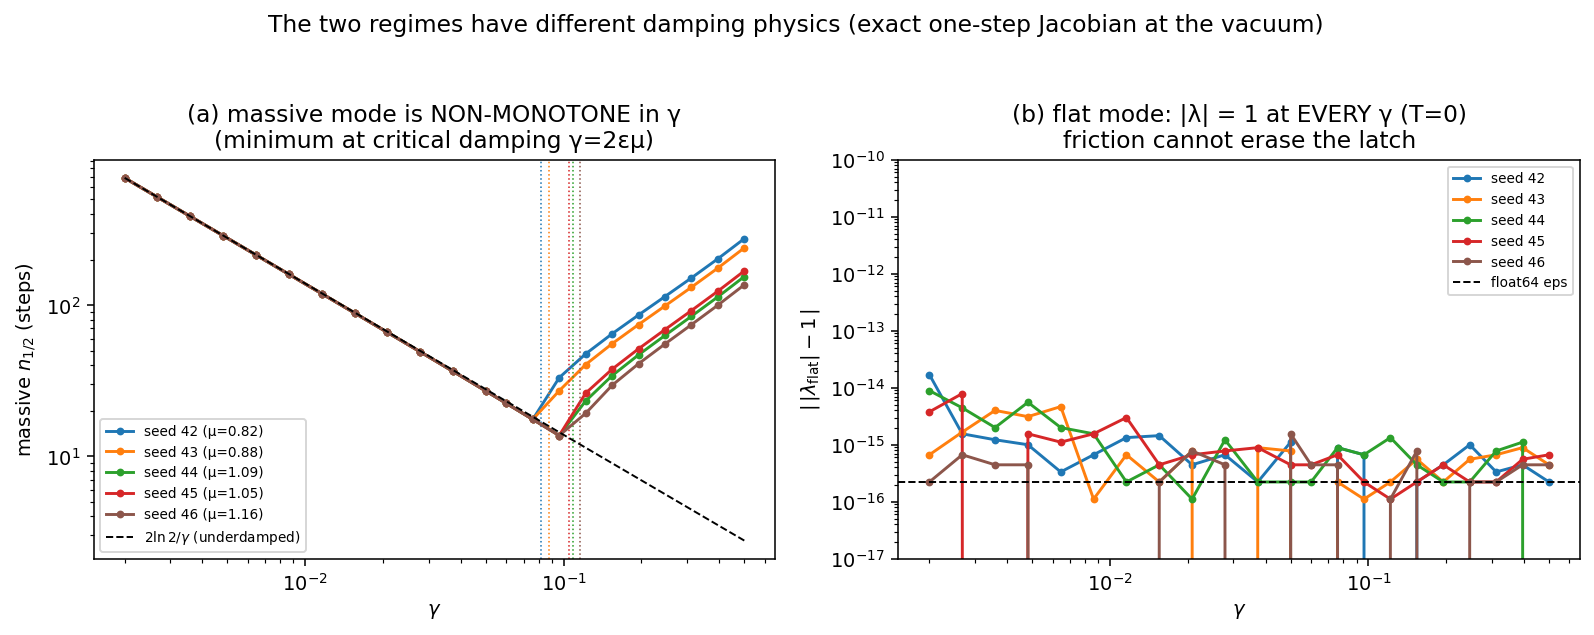
\includegraphics[width=\linewidth]{figs/figB_massive_vs_flat.png}
\caption{The two regimes, read off the exact one-step Jacobian at the vacuum. (a) The massive radial mode is non-monotone in $\gamma$, each seed's minimum sitting at its own $\gamma_{\rm crit}=2\varepsilon\mu$ (dotted), against the dashed underdamped envelope $2\ln2/\gamma$ drawn on the same axes. (b) The flat mode holds $|\lambda|=1$ at every $\gamma$ to the float64 floor: friction cannot erase the latch. \emph{Five trained designed seeds, $T=0$, dim 4, hidden 64, $\varepsilon=0.05$, single-CPU: verification.}}
\label{fig:massiveflat}
\end{figure}

\section{The Emergent Arm, and the V-Curve on a Second Instrument}\label{app:emergent}

\begin{figure}[!htb]
\centering
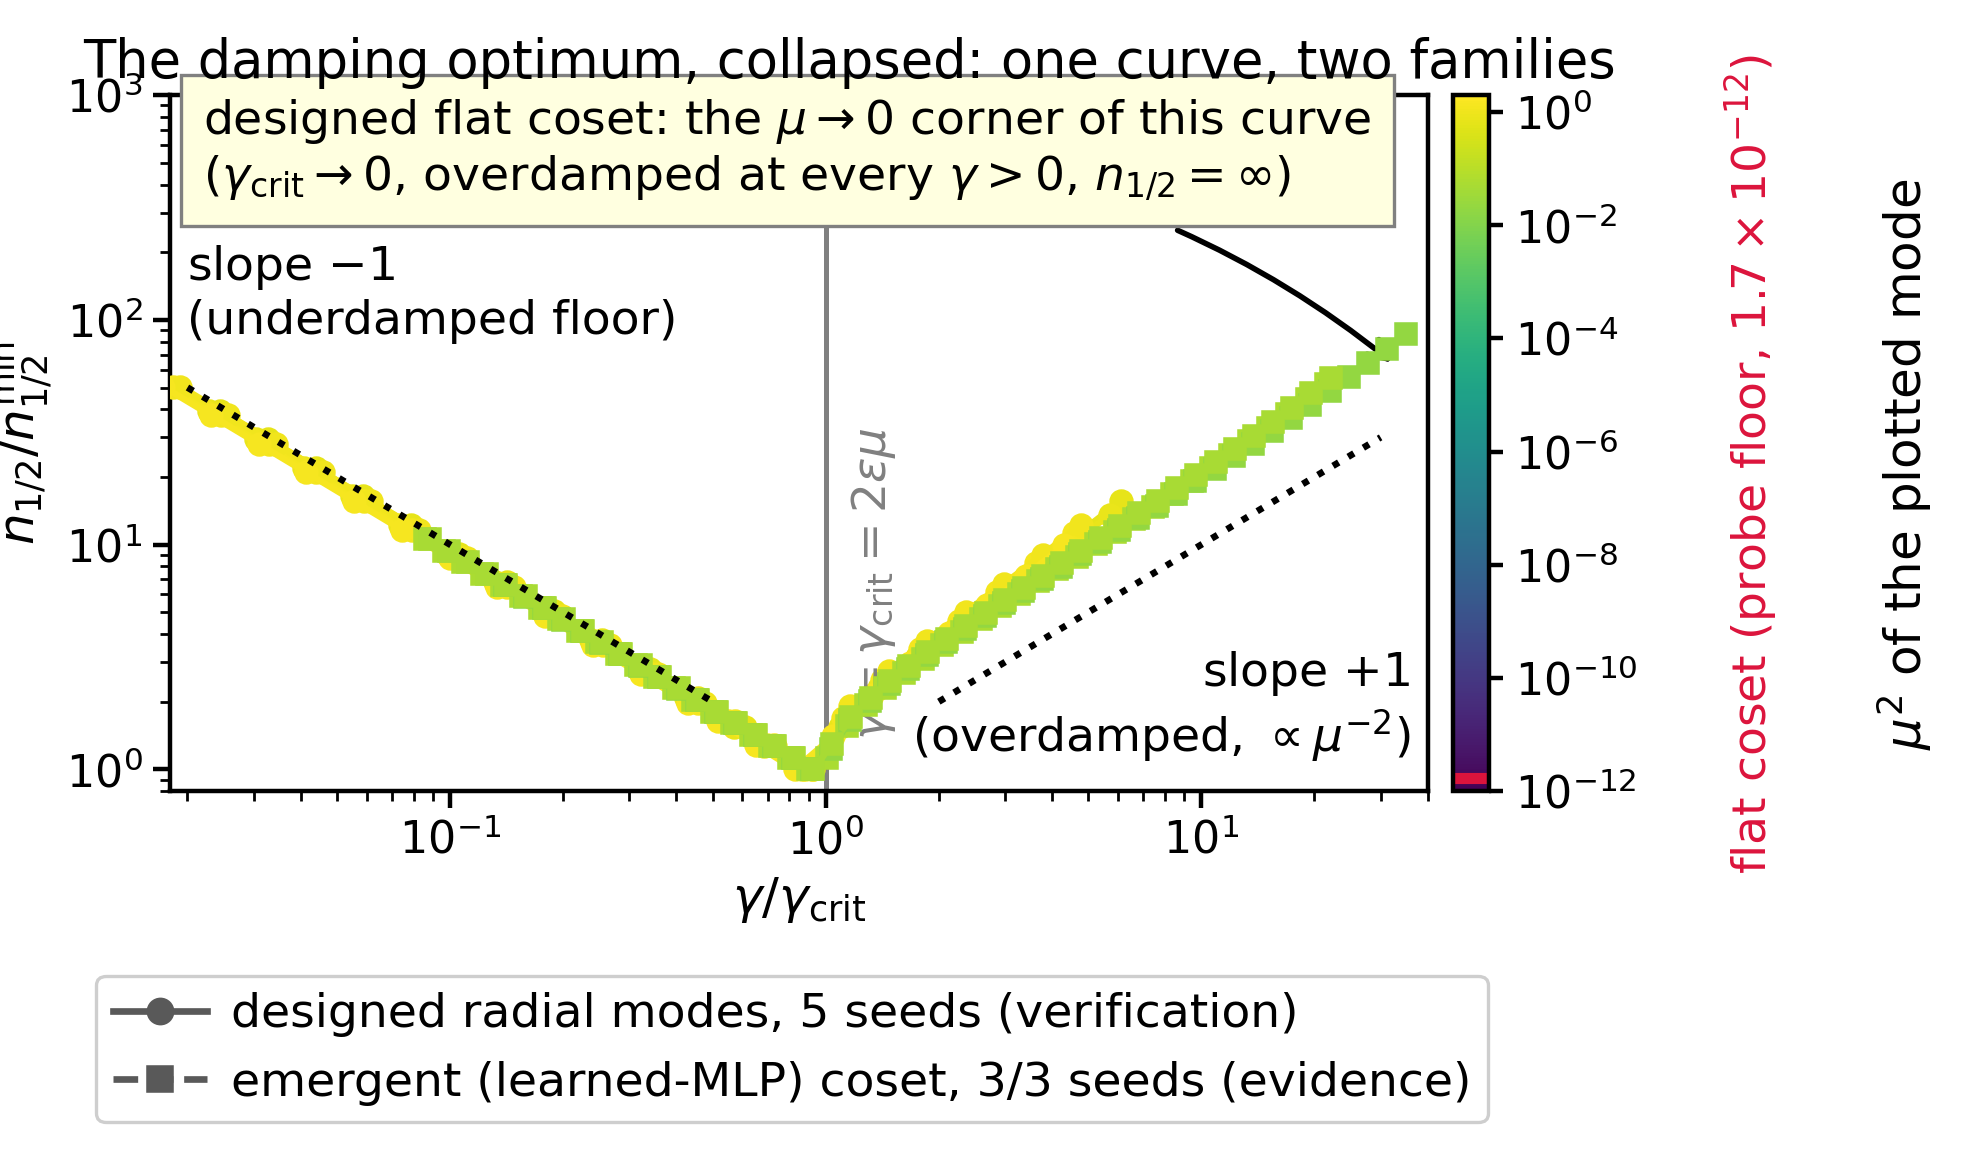
\includegraphics[width=\linewidth]{figs/figA1_damping_optimum_full.png}
\caption{\emph{The damping optimum, collapsed: the full-size version of Figure~\ref{fig:collapse}.} The same eight measured curves and the same $\mp1$ asymptotes, carrying the annotations the main-text version omits: the two-family legend, the $\gamma=\gamma_{\rm crit}=2\varepsilon\mu$ marker, the $\mu\to0$ flat-coset callout, and the crimson probe-floor tick on the $\mu^2$ colorbar ($1.7\times10^{-12}$). No plotted value differs from Figure~\ref{fig:collapse}. \emph{(One-step Jacobian; dim 4, hidden 64, $\varepsilon=0.05$, single-CPU; \texttt{langevin\_noise="fdt"}, Newtonian kinetic mode.)}}
\label{fig:collapse-full}
\end{figure}

We evaluate the emergent MLP checkpoints utilizing 3 unique seeds alongside a precisely matched designed control. All predictions detailed below were structurally filed and pre-registered prior to the execution of any test harness, establishing rigorous evidence parameters.

We deploy four specific measurement instruments over identical fit windows (defined as $\gamma<\gamma_{\rm crit}/2.5$ and $\gamma>2.5\gamma_{\rm crit}$):
1.  \emph{I-J}: The exact one-step Jacobian, where $n_{1/2}=\ln2/(-\ln|\lambda_{\rm ret}|)$.
2.  \emph{I-R1}: The rollout first crossing threshold of $|\theta|\le\delta/2$.
3.  \emph{I-R2}: The rollout last crossing threshold.
4.  \emph{I-R3} (Primary): The rollout envelope-rate fit evaluated specifically over the late window, guaranteeing $R^2\ge0.9955$ (median $0.9996$) across every evaluated cell.

\begin{table}[!htb]\centering\small
\caption{The foundational shape claims evaluated on all four designated instruments ($\delta=0.05$ rad, exactly 48 $\gamma$ values, utilizing 3 emergent seeds). The rollout rate instrument reproduces the Jacobian; both threshold instruments fail below $\gamma_{\rm crit}$, so no rollout $n_{1/2}$ is ever quoted from a threshold there. Rows are stacked by quantity so that no column is truncated; no value differs from the per-instrument reading.}
\begin{tabular}{llcccc}
\toprule
Quantity & Instrument & Seed 42 & Seed 43 & Seed 44 & Mean $\pm$ sd\\
\midrule
$\gamma_{\rm crit}$ & --- & $0.02334$ & $0.01424$ & $0.02265$ & ---\\
\midrule
\multirow{4}{*}{Argmin$/\gamma_{\rm crit}$} & I-J & $0.8994$ & $0.9046$ & $0.9055$ & $0.9032\pm0.0027$\\
 & I-R1 & $0.0857$ & $0.1404$ & $0.0883$ & $0.1048\pm0.0252$\\
 & I-R2 & $0.2068$ & $0.1404$ & $0.3031$ & $0.2168\pm0.0668$\\
 & I-R3 & $0.8928$ & $0.9047$ & $0.9028$ & $0.9001\pm0.0052$\\
\midrule
\multirow{4}{*}{Slope Below} & I-J & $-1.0023$ & $-1.0016$ & $-1.0022$ & $-1.0020\pm0.0003$\\
 & I-R1 & $+0.0725$ & $+0.0688$ & $+0.0455$ & $+0.0623\pm0.0120$\\
 & I-R2 & $-1.0556$ & $+0.0688$ & $-0.8854$ & $-0.6240\pm0.4948$\\
 & I-R3 & $-0.9651$ & $-0.9977$ & $-0.9854$ & $-0.9827\pm0.0134$\\
\midrule
\multirow{4}{*}{Slope Above} & I-J & $+1.1262$ & $+1.1031$ & $+1.1254$ & $+1.1182\pm0.0107$\\
 & I-R1 & $+1.1027$ & $+1.0889$ & $+1.0977$ & $+1.0964\pm0.0057$\\
 & I-R2 & $+1.1027$ & $+1.0889$ & $+1.0977$ & $+1.0964\pm0.0057$\\
 & I-R3 & $+1.1255$ & $+1.1030$ & $+1.1231$ & $+1.1172\pm0.0101$\\
\bottomrule
\end{tabular}
\end{table}

\paragraph{Instrument Level Disparities:} On the strictly overdamped branch ($\gamma\ge2\gamma_{\rm crit}$), the physical decay \emph{rates} match perfectly, whereas the \emph{threshold} instrument is consistently offset by an exact per-checkpoint constant flat in relation to $\gamma$. The full-window value for Seed 44 measures $0.9216\pm0.0027$, sitting precisely $0.0004$ beneath its pre-registered bounds due to the residual presence of a secondary faster mode within the window. The primary cause of this threshold offset is confirmed: the ring write mechanism consistently deposits only a specific limited fraction of its absolute amplitude directly into the designated slow branch (envelope-fit intercept over $\delta$ measuring $0.638/0.644/0.327$).

\begin{table}[!htb]\centering\small
\caption{The instrument gap is a level, not a rate: on the overdamped branch ($\gamma\ge2\gamma_{\rm crit}$) the decay \emph{rates} agree while the \emph{threshold} instrument is offset by a per-checkpoint constant flat in $\gamma$. Seed 44's full-window value ($0.9216\pm0.0027$) sits $0.0004$ below its pre-registered band because that window still contains a second, faster mode (early-window ratio $0.539$); the window-split diagnostic converges monotonically to $1$ into the asymptote. Cause of the threshold offset, measured: the ring write deposits only a fraction of its amplitude in the slow branch (envelope-fit intercept over $\delta$ = $0.638/0.644/0.327$).}
\begin{tabular}{p{0.06\linewidth}p{0.25\linewidth}p{0.22\linewidth}p{0.30\linewidth}}
\toprule
seed & $\Gamma_{\rm jac}/\Gamma_{\rm R3}$ (asymptotic window) & $n_{\rm jac}/n_{\rm R1}$ (threshold) & CV of $n_{\rm jac}/n_{\rm R1}$ over the grid\\
\midrule
42 & $0.9935$ & $1.3307$ & \multirow{3}{*}{$2.2$--$3.7\%$ over 21--25 $\gamma$-points}\\
43 & $1.0000$ & $1.7981$ & \\
44 & $0.9948$ & $1.8204$ & \\
\midrule
mean & $0.995\pm0.003$ & per seed, at $\delta=0.05$ rad & $|d\log(\text{ratio})/d\log\gamma|\le0.0034$ (threshold $0.10$)\\
\bottomrule
\end{tabular}
\end{table}

\paragraph{Finite Write Amplitudes:} At the specific values $\delta=0.05/0.2/0.5$ rad, the designated I-R3 argmin logs at $0.8928/0.9007/0.8968$ (seed 42), $0.9047/0.9045/0.9174$ (seed 43), and $0.9028/0.9037/0.9070$ (seed 44). This variance accounts for a maximum shift of $+1.4\%$ across a complete order of magnitude ($10\times$ range), with identical slope variances constrained strictly beneath $1.9\%$. Every iteration at $\delta=0.5$ relaxed identically to absolute baseline ($|\theta_{\rm final}|\le6.5\times10^{-10}$), preventing any seed's write function from clearing its designated washboard barrier.

\paragraph{Left Branch Exclusions:} For conditions where $\gamma<\gamma_{\rm crit}$, the respective coset eigenpair fundamentally becomes complex with $|\lambda|^2=1-\gamma$. This forces $n_{1/2}=\ln2/(-\tfrac12\ln(1-\gamma))$ to operate entirely independent of both $\mu^2$ and the specific architectural checkpoint. For instance, at exactly $\gamma=0.002$, emergent seeds 42 ($\mu^2=5.449\times10^{-2}$) and 43 ($\mu^2=2.029\times10^{-2}$) return identical metrics: $\lambda_{\rm ret}=0.998999499$ alongside an $n_{1/2}$ of $692.5$, aligning tightly against the calculated $2\ln2/0.002=693.1$.

\begin{figure}[htbp]
  \centering
  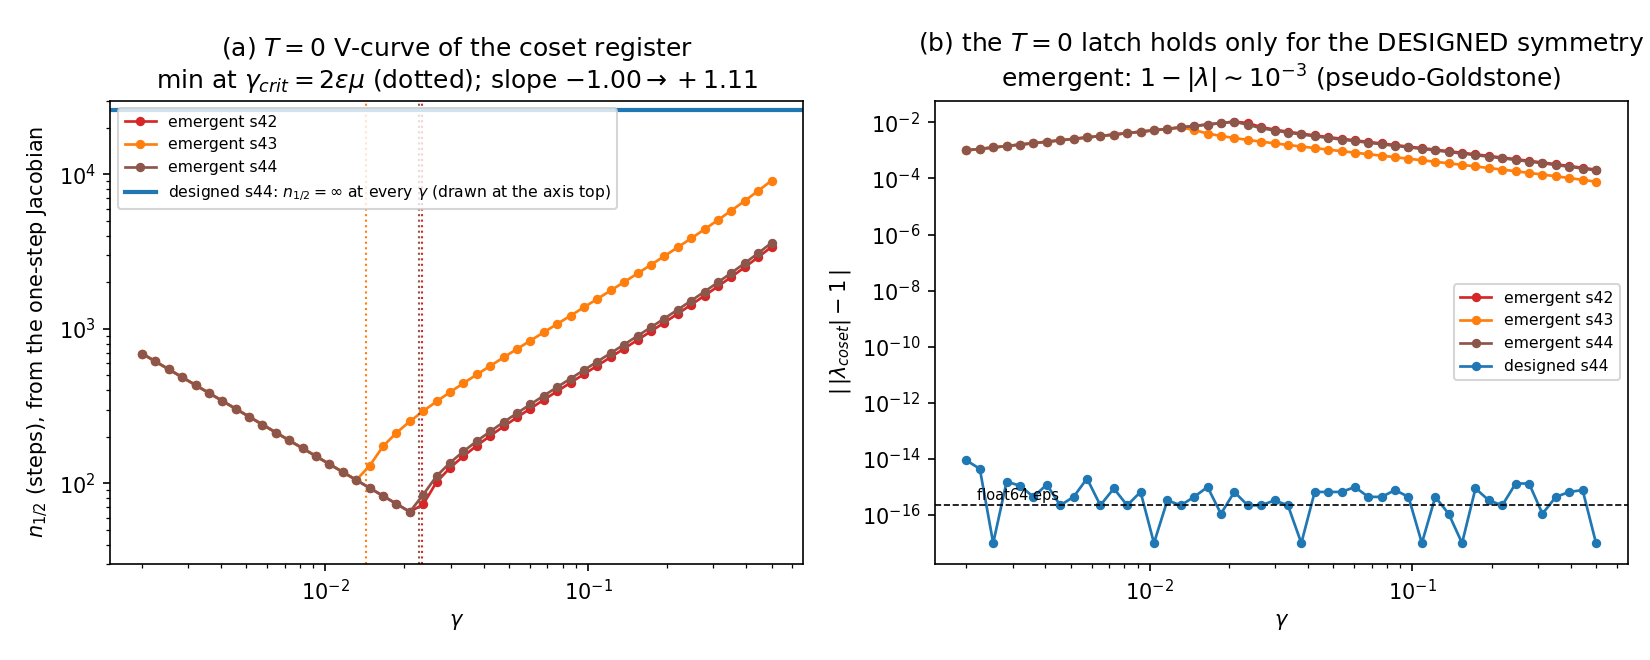
\includegraphics[width=\linewidth]{figs/figC_lambda_coset.png}
  \caption{The exact emergent V-curve depicted un-collapsed, outlining the distinct negative baseline parameters beside it. (a) Displays the precise $T=0$ half-life charted against friction for each separate emergent seed compiled from the one-step Jacobian. (b) Tracks $\big||\lambda_{\rm coset}|-1\big|$, revealing exact floor alignment for the strictly designed symmetry but falling short by precisely $\sim10^{-3}$ on all emergent seeds. \emph{Evaluated using three emergent MLP seeds against one rigidly matched designed control.}}
  \label{fig:lambdacoset}
\end{figure}

\begin{figure}[htbp]\centering
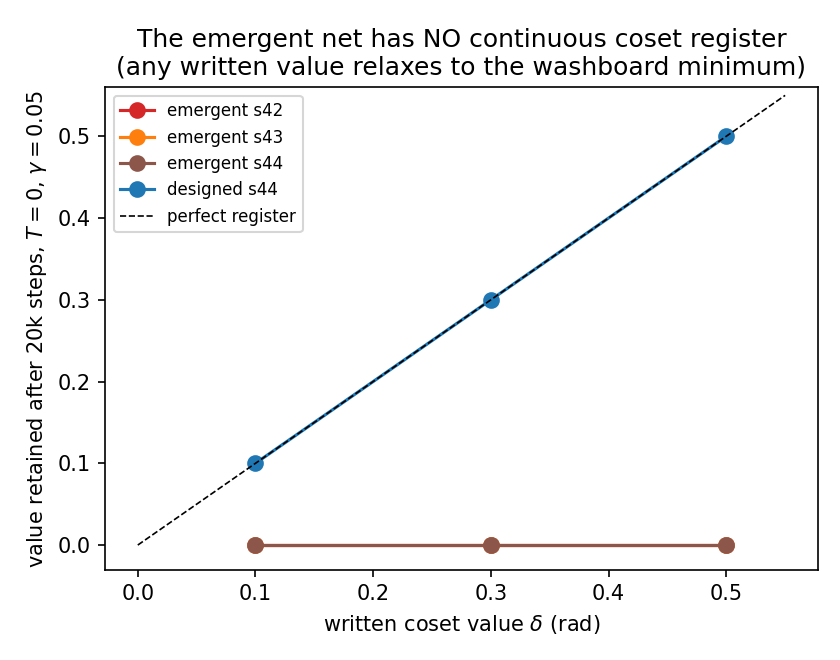
\includegraphics[width=\linewidth]{figs/figC_register_capacity.png}
\caption{The emergent unit has no continuous coset register. A written coset value $\delta$ is held for $20\,000$ steps at $T=0$, $\gamma=0.05$: on every emergent seed the value relaxes to the washboard minimum and nothing is retained, where the designed checkpoint returns $\delta$ exactly. \emph{Three emergent MLP seeds plus a matched designed control: evidence.} This is the figure behind the capacity statement of $\approx1$--$1.6$ bits.}
\label{fig:registercapacity}
\end{figure}

\begin{figure}[htbp]\centering
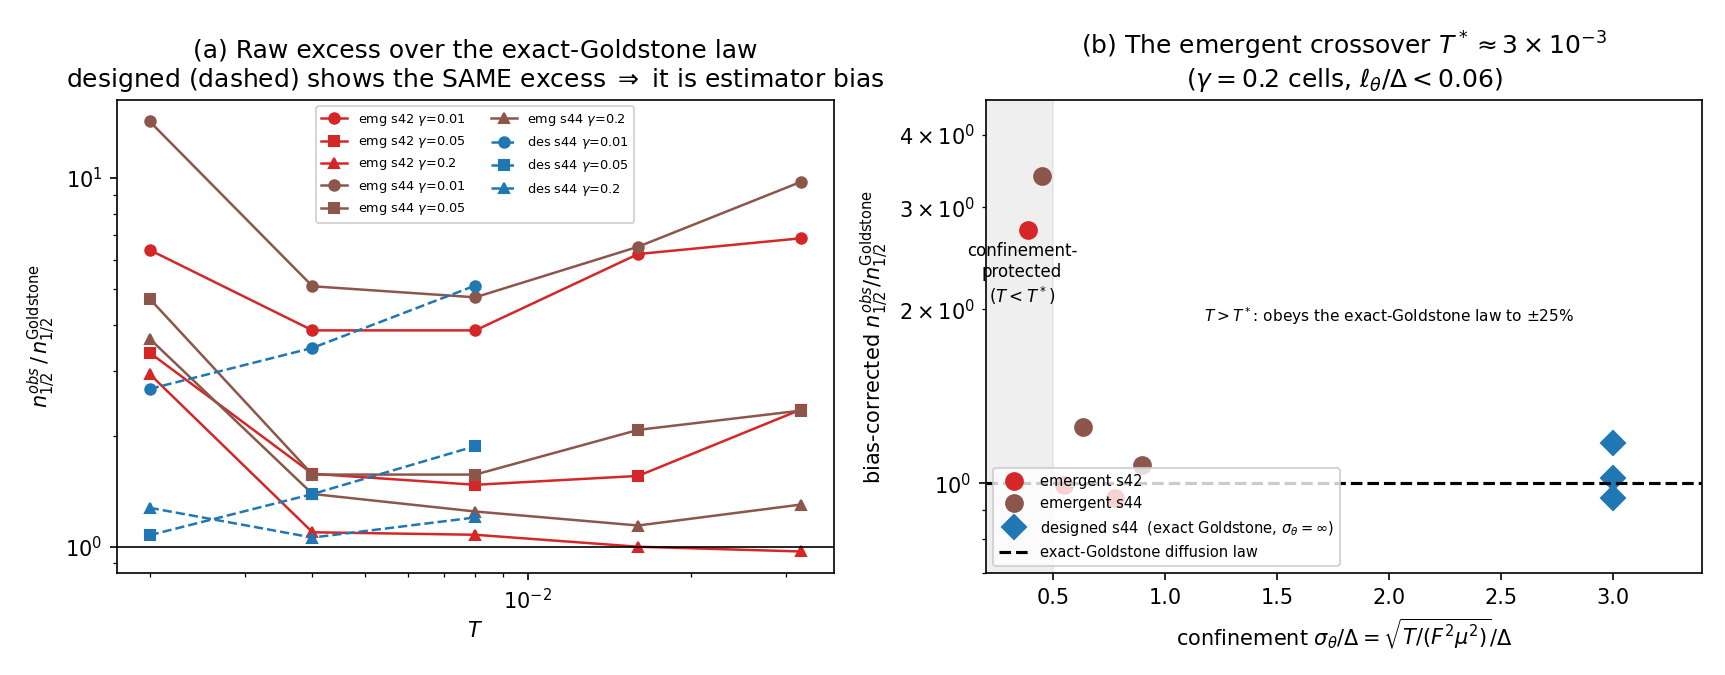
\includegraphics[width=\linewidth]{figs/figC_Tstar.png}
\caption{The crossover $T^\star$, and why the raw curve cannot be read directly. (a) The raw excess over the exact-Goldstone law is the same on the matched designed control as on the emergent seeds, so the excess is estimator bias rather than physics. (b) Bias-corrected, the emergent coset joins the exact-Goldstone law above $T^\star\approx3\times10^{-3}$, the shaded band being the confinement-protected cells below it. \emph{Multi-seed status, stated plainly: two emergent seeds and one matched designed control, an $n<3$ cell.} $\Delta=0.5$ rad, $\ell_\theta/\Delta<0.06$, \texttt{langevin\_noise="fdt"}, Newtonian kinetic mode: evidence.}
\label{fig:tstar}
\end{figure}

\begin{figure}[!htb]
\centering
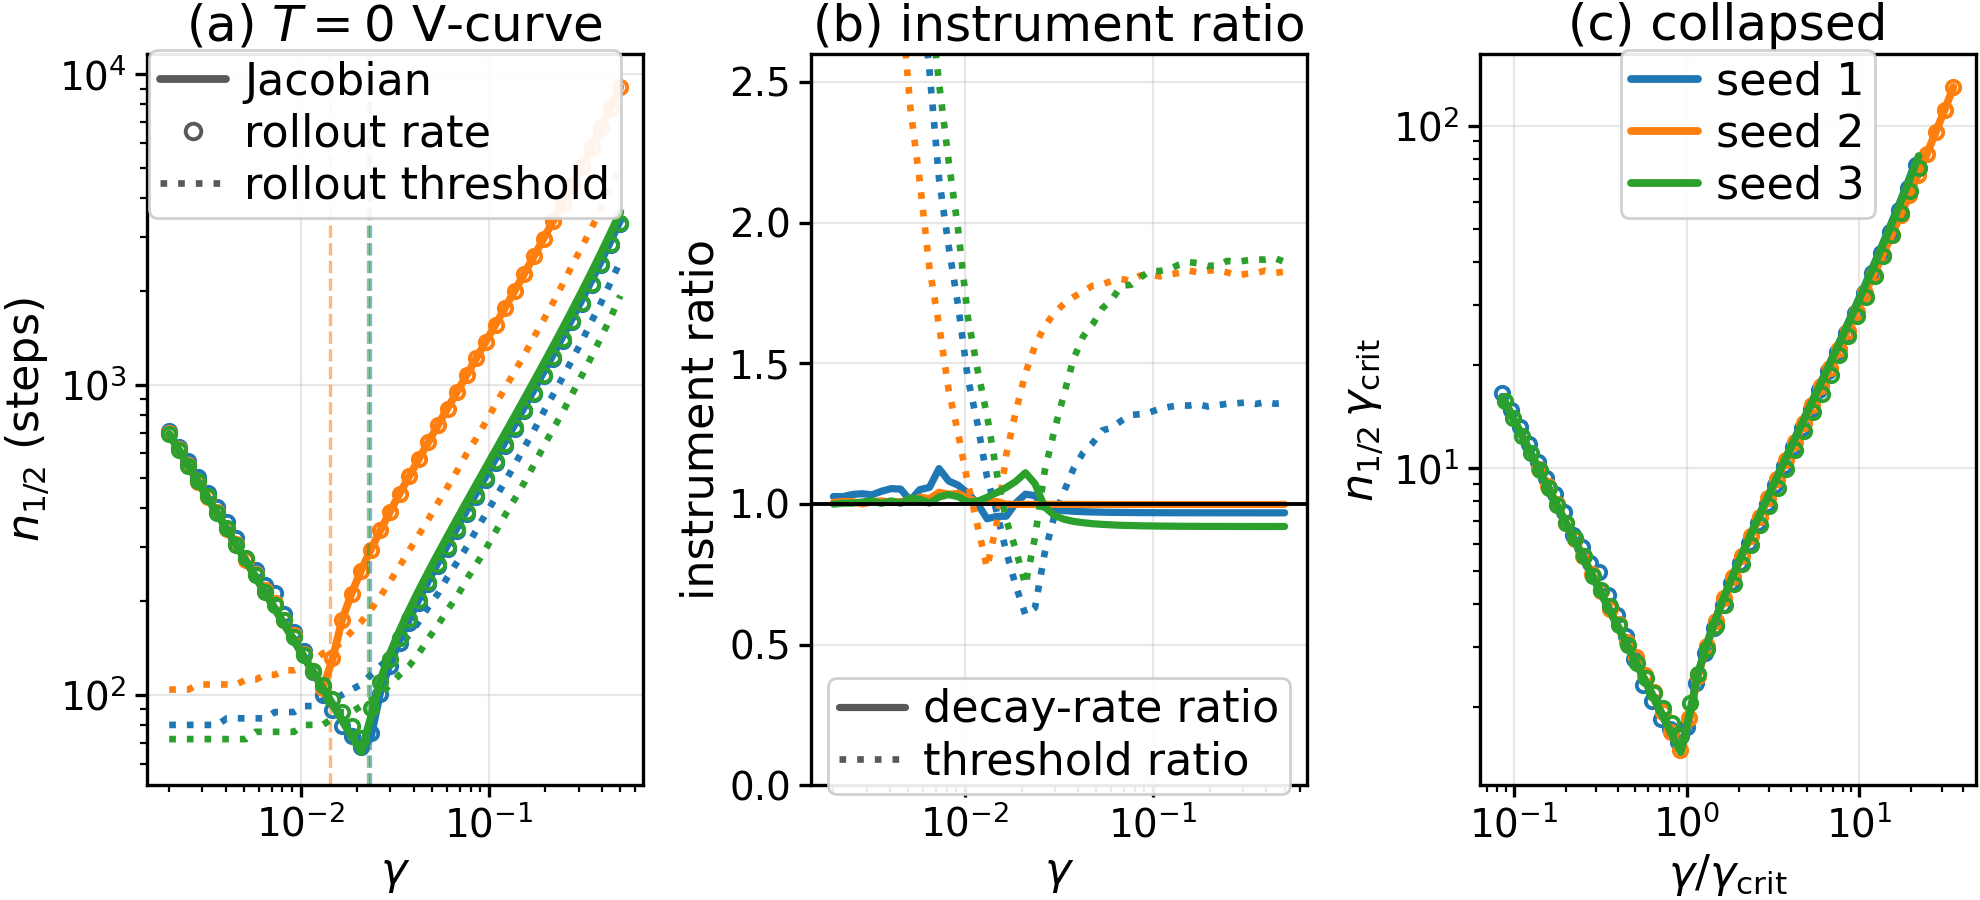
\includegraphics[width=\linewidth]{figs/fig2_two_instruments.png}
\caption{The V-curve measured a second way. (a) $T=0$ $n_{1/2}(\gamma)$ per emergent seed on the one-step Jacobian (I-J, lines), the rollout envelope-rate instrument (I-R3, circles) and the rollout first-crossing threshold (I-R1, dotted), at $\delta=0.05$ rad. (b) The per-$\gamma$ instrument ratio: the rate ratio sits on $1$, the threshold ratio is offset and flat in $\gamma$ above $\gamma_{\rm crit}$. (c) The same data in collapsed variables. \emph{(Emergent MLP, 3 seeds, dim 4, hidden 64, $\varepsilon=0.05$, float64, $T=0$, pre-registered $\Rightarrow$ evidence.)}}
\label{fig:twoinstruments}
\end{figure}

\section{The Friction-Hole Vault, on Both Arms}\label{app:vault}

This mechanism dictates that the shipped field remains strictly absorb-only, following $p\leftarrow(1-\gamma_\phi)(1-\gamma)p+\sigma(\gamma)\xi$ with $\sigma^2=MT\gamma(2-\gamma)$. This is dictated strictly by the \emph{scalar} $\gamma$, yielding parameters $\gamma_{\rm eff}=1-(1-\gamma)(1-\gamma_\phi)$, $T_{\rm local}=T\gamma(2-\gamma)/[\gamma_{\rm eff}(2-\gamma_{\rm eff})]$ and importantly $D_\theta=\varepsilon T\gamma(2-\gamma)/(2F^2\gamma_{\rm eff}^2)$. The resulting vault effectively computes to $(\gamma_{\rm eff}/\gamma)^2$. Conversely, a coupled bath alternative would dictate $D_\theta\propto\gamma_{\rm eff}^{-1}$ returning a vault of $13.88\times$ exactly at $\gamma=0.05$, $\gamma_\phi=0.5$. These competing hypotheses scale apart by a factor of $7.942\times$; experimental results comprehensively refute the coupled-bath prediction.

\paragraph{Designed Arm Assessment:} We observe $\mathrm{Var}(p_i)/(M_iT)=0.9986$ at baseline ($\gamma_\phi=0$), scaling to $0.36171\pm0.00129$ at ($0.1$), $0.23044$ at ($0.2$), $0.17513$ at ($0.3$), and definitively hitting $0.12600\pm0.00031$ at ($0.5$). This closely mirrors the pure absorb prediction of $0.12591$. Consequently, $T_{\rm local}$ drops precisely to $1.26\times10^{-4}$, equating to a $7.94\times$ functioning refrigerator effect. The comprehensive $D_\theta$-based structural vault records exponential factors of $8.42\times$, $22.39\times$, $44.31\times$, and finally $107.77\pm4.78\times$ specifically at $\gamma_\phi=0.1/0.2/0.3/0.5$ (matching the absorb baseline prediction of $110.25$). Conversely, the scalar control isolated at identical $\gamma_{\rm eff}$ reads merely $13.28\pm0.12\times$. At true absolute zero ($T=0$), the hole functionally erases absolutely nothing, logging drift boundaries of strictly $\le1.75\times10^{-12}$ rad per 200k continuous execution steps inside and out.

\paragraph{Emergent Arm Translation:} Since the structural coset here is definitionally bounded ($\mu^2_{\rm adiab}=2.77\times10^{-2}$ to $8.93\times10^{-2}$), the baseline designed block estimator is biased artificially low by nearly $55\%$. It is therefore systematically replaced by a rigorously cross-validated, window-free Ornstein--Uhlenbeck fit parameter measuring $\mathrm{MSD}(n)=A(1-e^{-n/\tau})$ and $\hat D=A/(2\varepsilon\tau)$. On the strictly bounded evaluation cells, the law-referenced absolute vault computes successfully to $106.1\pm5.0\times$ against the fundamental prediction of $110.25\times$. The contrast metric, however, remains uniquely native to the designed architecture: the measured field-to-scalar control variance computes to $23.39\pm10.06$ against a pre-registered bounds parameter of $[6.5,9.5]$, triggering the designated falsifier constraint strictly because the control arm intrinsically delocalizes while the main field functionally adheres to the absorb limit.

\begin{table}[!htb]\centering
\caption{The refrigerator law transfers exactly to an emergent register: $\mathrm{Var}(p_i)/(M_iT)$ against the absorb-only prediction, 2048 walkers $\times$ 40 samples, 3 emergent seeds; over all 24 field cells observed/absorb $=0.9998\pm0.0019$, and at $\gamma_\phi=0.5$ $T_{\rm local}/T=0.12570$, a $7.955\times$ refrigerator against $7.942$ predicted. The coupled bath predicts $1.0$ everywhere and is measured at $0.2235$.}
\begin{tabular}{lcccccc}
\toprule
$T$ & $\gamma_\phi$ & $\gamma_{\rm eff}$ & absorb pred. & coupled pred. & measured & obs/absorb\\
\midrule
$4\times10^{-3}$ & $0.0$ & $0.050$ & $1.00000$ & $1.0$ & $0.99815\pm0.00257$ & $0.9981$\\
$4\times10^{-3}$ & $0.1$ & $0.145$ & $0.36249$ & $1.0$ & $0.36326\pm0.00067$ & $1.0021$\\
$4\times10^{-3}$ & $0.2$ & $0.240$ & $0.23082$ & $1.0$ & $0.23062\pm0.00080$ & $0.9991$\\
$4\times10^{-3}$ & $0.3$ & $0.335$ & $0.17480$ & $1.0$ & $0.17473\pm0.00046$ & $0.9996$\\
$4\times10^{-3}$ & $0.5$ & $0.525$ & $0.12591$ & $1.0$ & $0.12592\pm0.00055$ & $1.0001$\\
$8\times10^{-3}$ & $0.5$ & $0.525$ & $0.12591$ & $1.0$ & $0.12548\pm0.00032$ & $0.9966$\\
\bottomrule
\end{tabular}
\end{table}

\begin{table}[!htb]\centering\small
\caption{The hole confines an emergent register, and the laundering control shows friction alone does not. $T=4\times10^{-3}$, 1024 walkers, burn-in $20\,000$--$80\,000$ steps, spread by interquartile range; ``hop'' means $|\theta|>1$ rad. The pre-registered stationary-spread comparison is \emph{void} here and no in/out spread ratio may be quoted from these checkpoints: the control that must return exactly $1.000$ returns $0.4586\pm0.1181$.}
\begin{tabular}{llccccc}
\toprule
seed & arm & $\gamma_{\rm eff}$ & $\sigma_\theta$ (IQR) & hop fraction & Boltzmann at $T_{\rm local}$ & obs/pred\\
\midrule
42 & no hole, $\gamma=0.05$ & $0.050$ & $0.40795$ & $5.50\%$ & $0.24073$ & $1.6946$\\
42 & scalar $0.525$ (control) & $0.525$ & $0.20034$ & $0.73\%$ & $0.24073$ & $0.8322$\\
42 & $\gamma_\phi$ hole & $0.525$ & $0.06442$ & $0.0000$ & $0.08542$ & $0.7542$\\
43 & no hole & $0.050$ & $1.17601$ & $42.97\%$ & $0.46059$ & $2.5533$\\
43 & scalar $0.525$ & $0.525$ & $0.35335$ & $10.20\%$ & $0.46059$ & $0.7672$\\
43 & $\gamma_\phi$ hole & $0.525$ & $0.08628$ & $0.0000$ & $0.16343$ & $0.5279$\\
44 & no hole & $0.050$ & $0.36922$ & $2.36\%$ & $0.24034$ & $1.5363$\\
44 & scalar $0.525$ & $0.525$ & $0.21574$ & $0.26\%$ & $0.24034$ & $0.8977$\\
44 & $\gamma_\phi$ hole & $0.525$ & $0.07279$ & $0.0000$ & $0.08528$ & $0.8535$\\
\bottomrule
\end{tabular}
\end{table}

\begin{figure}[!htb]
\centering
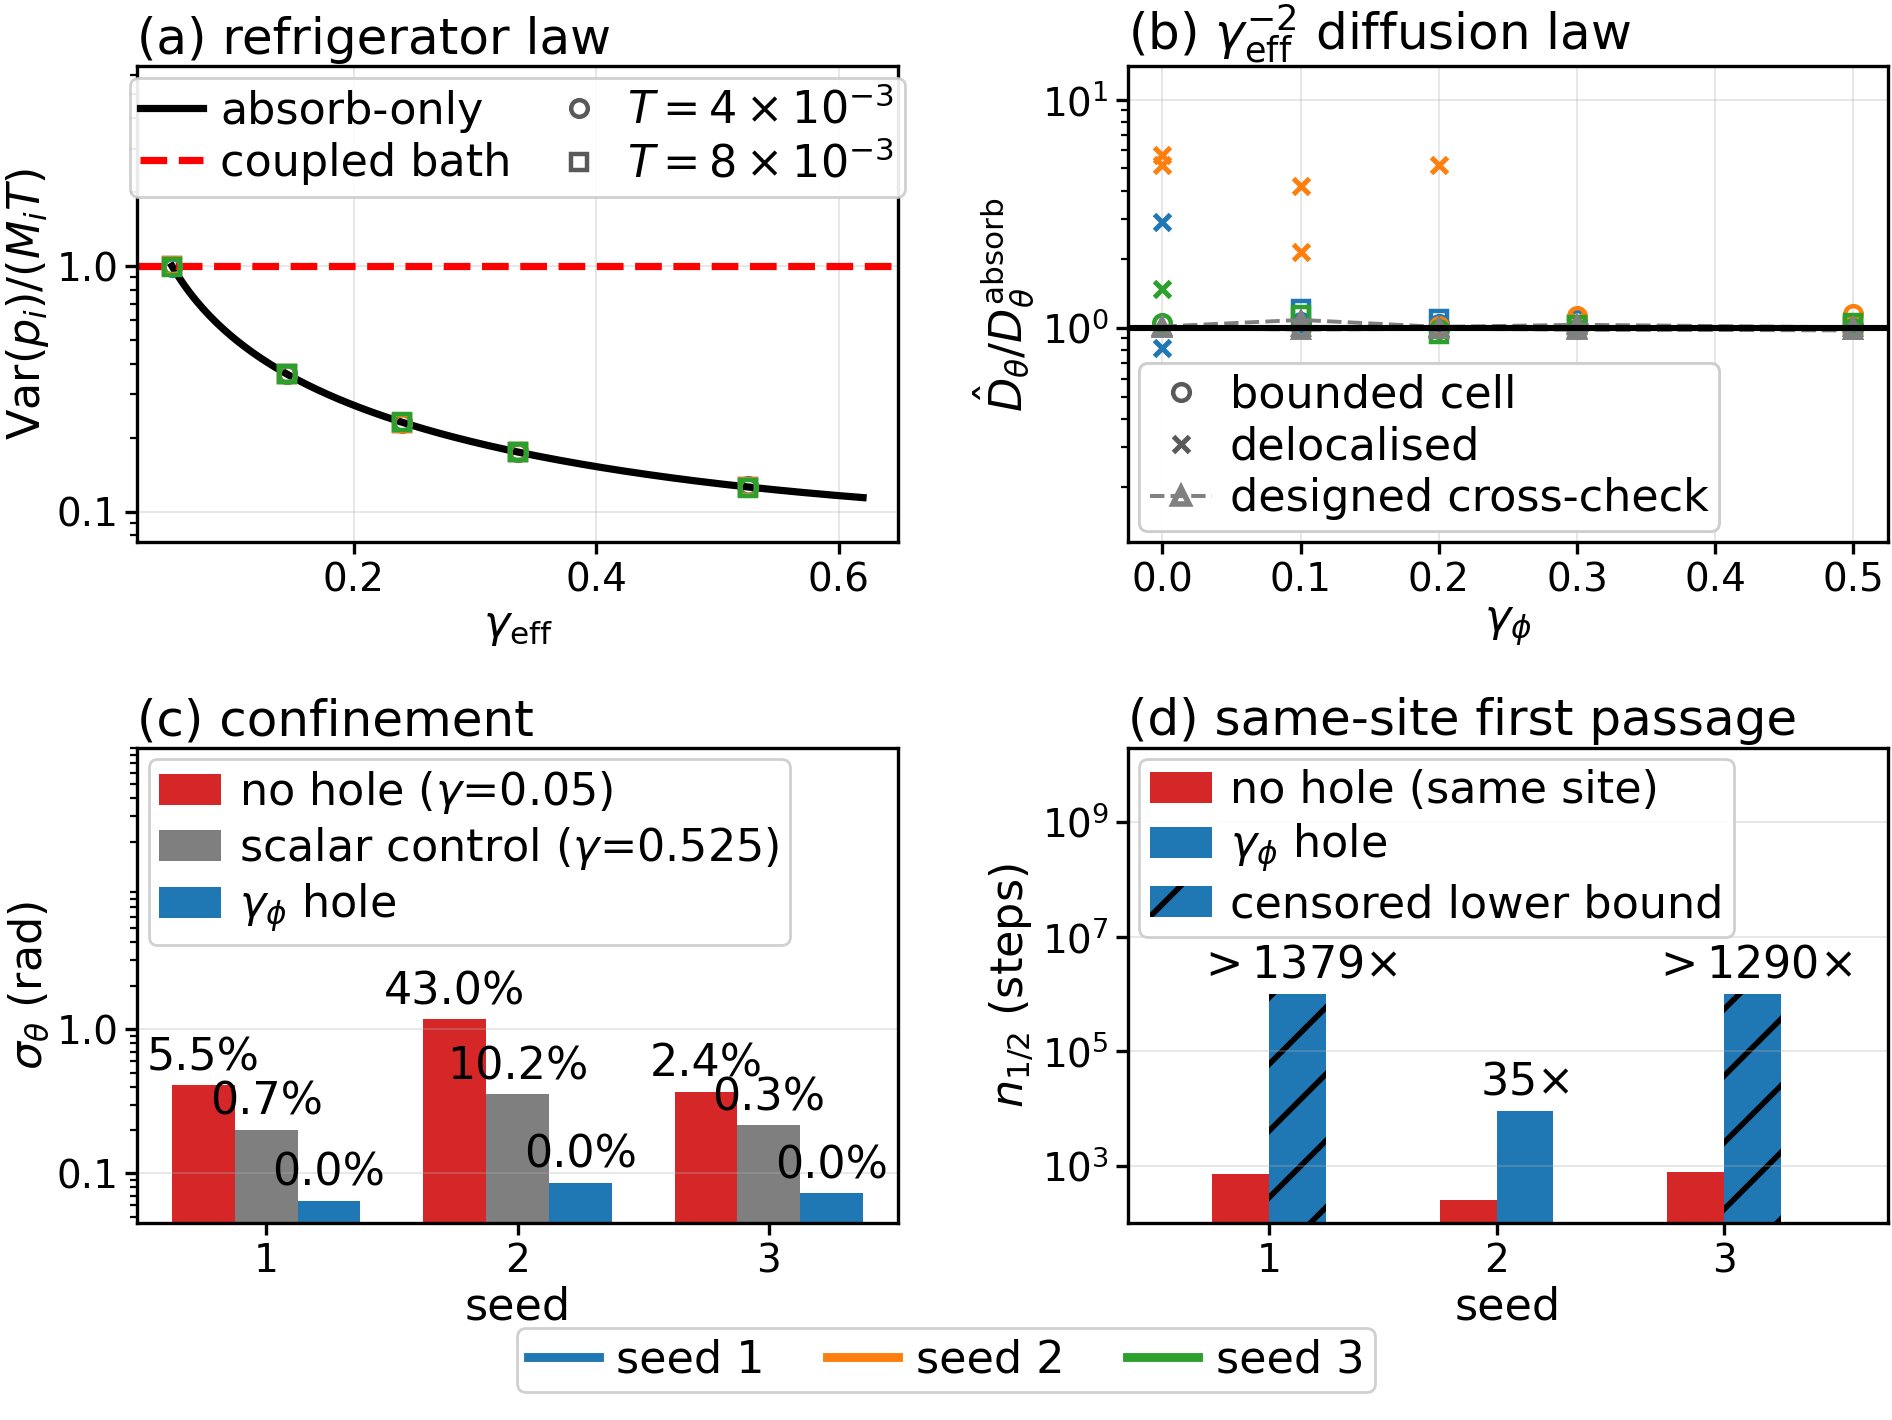
\includegraphics[width=\linewidth]{figs/figC2_vault_emergent.png}
\caption{The vault on an emergent register; panels are labeled by the pre-registered prediction each tests. (a) The refrigerator law, $\mathrm{Var}(p_i)/(M_iT)$ against $\gamma_{\rm eff}$ for 3 seeds $\times$ 2 temperatures, on the absorb-only curve with the coupled-bath prediction (dashed) rejected. (b) The $\gamma_{\rm eff}^{-2}$ diffusion law: bounded cells as circles and squares, delocalized cells as crosses, the designed cross-check overlaid. (c) Confinement: stationary spread and hop fraction for no hole, the scalar control and the hole. (d) Same-site first passage; hatched bars are censored lower bounds. \emph{(Emergent MLP, 3 seeds, $T\in\{4,8\}\times10^{-3}$, both above $T^\star$, $\Delta=0.5$ rad.)}}
\label{fig:vault-emergent}
\end{figure}

\section{Exact Store-Level Deletion: Prior Work and Measured Tables}\label{app:deletion}

\paragraph{Prior Work:} Uniquely represented (canonical) data structures date to \citet{snyder_uniquely_1977} and \citet{andersson_new_1995}; \emph{obliviousness}, a distributional condition on the memory representation which explicitly does not require canonical representation, is \citeauthor{micciancio_oblivious_1997}'s \citeyearpar{micciancio_oblivious_1997}; the weak and strong history-independence notions used here are \citeauthor{naor_anti-persistence_2001}'s \citeyearpar{naor_anti-persistence_2001}; the open-addressed realization is \citeauthor{blelloch_strongly_2007}'s \citeyearpar{blelloch_strongly_2007}, whose table is a stable matching between keys and slots under a global key priority, and it is that priority-greedy rule and that delete-time fix-up cascade we use; \citet{hutchison_uniquely_2008} had already taken unique representation into computational geometry. We claim no priority over order-independent placement and no novelty for the displacement rule or its delete-time repair. New is the composition: slots that are a lattice packing, so the canonical representation carries a minimum-separation certificate; content that is a continuously decaying amplitude whose decay commutes with deletion; a canonical object that is an energy function a dynamical read relaxes into; and a price that is negative where strong history independence is known to cost as much as an exponential slowdown relative to the weak notion for comparison-based structures \citep{goos_lower_2003}. ``Fix-up cascade'' is our name for the \texttt{NEXT}-chain delete-time repair of their Figure 1; the algorithm is theirs either way.

\paragraph{Structural Exactness at Zero Tolerance:} The architectural implementation dictates 24 exhaustive structural orders explicitly measured at $n=4$, mapped alongside 200 independently randomized sequence orders strictly at $n\in\{8,16,40,64\}$. Furthermore, we implement 100 dedicated write/delete functional interleavings and absolute mid-decay continuous deletes. Across every evaluation parameter, the resulting structural spacing enforces an exact boundary of $1.540000$. On the subsequently shipped operational store architecture, the structural centers, exact payloads, physical amplitudes, and the defining active logic mask are unconditionally byte-equal, with the energy profile $V(q)$ proving purely byte-equal across 64 heavily randomized direct queries.

\paragraph{The Negative Packing Price Constraint:} Evaluated precisely at the defined ceiling $K=64$, the purely canonical stable-matching rule structurally admits exactly $61/64$ actively offered sequential keys deterministically ($\sigma=0$, per-offered index of $0.9531$). This ratio actively climbs to absolute capacity ($64/64$) once physical lattice sizing is symmetrically inflated by an exactly specified coefficient of $\times1.05$. By contrast, the stochastic refuse-and-relocate allocator architecture solely manages to admit exactly $43/64$ operating on those perfectly identical geometric seeds (per-offered logic ceiling of $0.6719$). It must be firmly stated that at peak physical overflow limit, operating totally independently without the waitlist active, structural exactness completely and predictably collapses: analyzing exactly 7 baseline cells receiving 8 strict capacity offers, $\mathrm{AUC}(n_{\rm live})$ returns $1.00000\pm0.0000$ and the functional byte-equal architectural fraction plummets directly to $0.0000$.

\begin{table}[!htb]\centering\small
\caption{The laundering control validation execution. Executed explicitly on the designed store featuring the shipped two-phase read geometry; evaluating 8 active targets against 3 separate seeds, mapping exactly 128 paired environments per target across 18 separate continuous amplitude limits.}
\begin{tabular}{p{0.34\linewidth}p{0.15\linewidth}p{0.19\linewidth}p{0.16\linewidth}}
\toprule
Evaluated Adversary Model & Physical Decay & TTL Flag Limit (Same Store) & Resolution Separation\\
\midrule
White-box architecture, fully exact & $1.000$ & $1.000$ & $0.000$\\
Query-level membership depth, fully exact & $0.983$ & $1.000$ & $0.017$\\
Query-level membership depth, $\sigma_{\rm obs}=0.1$ & $0.559$ & $0.996$ & $0.437$\\
\bottomrule
\end{tabular}
\end{table}

\paragraph{Trilemma Parameters and Cost Evaluation:} The physically shipped final store structure completely abandons amplitude-independent baseline address limits, generating a strict operational lifetime correlation factor computed at exactly $r=-0.85$ scaling with $a_i^2$. We rigorously refute both standard previously proposed baseline repair variants: directly multiplying absolute payloads exponentially by their matched amplitudes completely corrupts the core value index criterion measured strictly at $A=1-\text{tol}/|a_i|$ (generating hard death physical amplitudes of exactly $0.90/0.80/0.70/0.30$). \emph{Retrieval geometry:} $R_{50}$ contracts $1.146/1.083/0.979/0.874/0.752$ as $A:1\to0.5\to0.2\to0.1\to0.06$, a $1.52\times$ contraction from $1.146\to0.752$, matching the pre-registered saddle prediction at all five points ($\pm0.20$), where a TTL vector store's lookup radius is a constant hard step at $0.75$--$0.77$, independent of age. Consequently, operating beneath the rigid barrier of its internal logic flag, the designated gated execution channel actively contracts the geometric value $R_{50}$ from $1.135\to0.771$. Note crucially that we define no explicit deletion-cost execution statement because the core canonical synchronization mandates a complete and structural $O(n)$ rebuild evaluated entirely per operation.

\section{Derivations of the Closed Forms}\label{app:derivation}

Every closed form asserted in Secs.~\ref{sec:vcurve}--\ref{sec:vault} and Apps.~\ref{app:budget}--\ref{app:vault} follows from a single object: the damped symplectic step, linearized about the vacuum. This appendix supplies the algebra; no result here is new, and each derivation terminates in exactly the form the text prints.

\paragraph{Assumptions.}
\begin{itemize}
\item \emph{The step.} One update is: half-kick $p\mapsto p-\tfrac{\varepsilon}{2}\nabla V_\theta(q)$; drift $q\mapsto q'=q+\varepsilon M^{-1}p$; half-kick at $q'$; damping $p\mapsto(1-\gamma)p$, position-gated by the further factor $\bigl(1-\gamma_\phi(q')\bigr)$ evaluated at the \emph{updated} position when a friction field is present; and, at $T>0$, additive noise $p\mapsto p+\sigma\xi$, $\xi\sim\mathcal N(0,I)$, in the Newtonian kinetic mode the Scope paragraph requires.
\item \emph{Linearization.} Retention statements expand $V_\theta$ to second order about the vacuum and diagonalize in the mass-whitened Hessian $M^{-1/2}\nabla^2V_\theta\,M^{-1/2}$, whose eigenvalues are the spectral masses $\mu_k^2$. Write $h=\varepsilon\mu$.
\item \emph{The coset scale $F$.} $F^2$ denotes the mass-weighted squared displacement of the latent state per unit of the stored coordinate: for a stored angle on a ring of radius $r_*$ with tied channel mass $M$, $F^2=M r_*^2$. Diffusion coefficients are per unit dynamical time $t=n\varepsilon$.
\end{itemize}

\subsection{The per-mode step matrix}\label{app:deriv:1} In a whitened normal-mode coordinate $(x,p)$ with $V=\tfrac12\mu^2x^2$, composing the four sub-steps above gives the linear map $\bigl(\begin{smallmatrix}x\\p\end{smallmatrix}\bigr)\mapsto J\bigl(\begin{smallmatrix}x\\p\end{smallmatrix}\bigr)$,
\[
J=\begin{pmatrix}1-\tfrac{h^2}{2} & \varepsilon\\[2pt] -(1-\gamma)\,\varepsilon\mu^2\bigl(1-\tfrac{h^2}{4}\bigr) & (1-\gamma)\bigl(1-\tfrac{h^2}{2}\bigr)\end{pmatrix},
\qquad
\operatorname{tr}J=(2-\gamma)\Bigl(1-\frac{h^2}{2}\Bigr),\quad \det J=1-\gamma .
\]
This is the ``entirely fixed by $(\varepsilon\mu,\gamma)$'' $2\times2$ matrix of the Methodological Foundations; its spectral radius sets each mode's retention.

\subsection{Conformal symplecticity}\label{app:deriv:2} The three Verlet sub-steps are shears (each Jacobian is triangular with unit diagonal), so their composition has determinant $1$. The damping sub-step is $q\mapsto q$, $p\mapsto(1-\gamma)p$, contributing $(1-\gamma)^d$; hence $\det J=(1-\gamma)^d$. The gate multiplies each momentum component by the scalar $\bigl(1-\gamma_\phi(q')\bigr)$; because $q'$ is already fixed when the gate acts, its Jacobian is block-triangular and contributes exactly $\bigl(1-\gamma_\phi(q')\bigr)^d$ --- the position-gated form quoted in Sec.~\ref{sec:vcurve}.

\subsection{The V-curve: two branches and $\gamma_{\rm crit}=2\varepsilon\mu$}\label{app:deriv:3} The eigenvalues of \ref{app:deriv:1} are $\lambda_\pm=\tfrac12\bigl(\operatorname{tr}J\pm\sqrt{\operatorname{tr}^2J-4\det J}\bigr)$, and the discriminant's sign splits the curve.

\emph{Underdamped branch} ($\operatorname{tr}^2J<4\det J$): the pair is complex with $|\lambda|^2=\det J=1-\gamma$, so
\[
n_{1/2}=\frac{\ln 2}{-\tfrac12\ln(1-\gamma)}\;\xrightarrow{\ \gamma\ll1\ }\;\frac{2\ln2}{\gamma},
\]
independent of $\mu^2$ and of the checkpoint --- the left-branch exclusion of App.~\ref{app:emergent} ($\lambda_{\rm ret}=\sqrt{1-0.002}=0.998999499$, $n_{1/2}=692.5$ vs.\ $2\ln2/0.002=693.1$), the dashed $2\ln2/\gamma$ envelope of Fig.~\ref{fig:massiveflat}a, and, evaluated at $\gamma=0.05$, the mass-independent floor of $27.03$ steps of App.~\ref{app:budget}.

\emph{Overdamped branch}: substituting $\lambda=1-\delta$ into $\lambda^2-\lambda\operatorname{tr}J+\det J=0$ gives exactly $\delta^2-\bigl[\gamma+(2-\gamma)\tfrac{h^2}{2}\bigr]\delta+(2-\gamma)\tfrac{h^2}{2}=0$, whose retained (slow) root is $\delta=(2-\gamma)h^2/(2\gamma)\,\bigl(1+O(h^2/\gamma^2)\bigr)$. Hence
\[
n_{1/2}=\frac{\ln2}{-\ln(1-\delta)}\;\simeq\;\frac{2\ln2\,\gamma}{(2-\gamma)\,\varepsilon^2\mu^2},
\]
the $\mu^{-2}$ law of Sec.~\ref{sec:vcurve}. Its log-slope is $d\ln n_{1/2}/d\ln\gamma=1+\gamma/(2-\gamma)$: it approaches the $+1$ asymptote only as $\gamma\to0$ and exceeds it at every finite $\gamma$, while the underdamped slope $-\gamma/[(1-\gamma)(-\ln(1-\gamma))]=-1-\tfrac{\gamma}{2}+O(\gamma^2)$ hugs $-1$ --- which is why the two measured branches are asymmetric (slopes near $-1$ below, $+1.1$ to $+1.3$ above, per the fit windows of Apps.~\ref{app:budget}--\ref{app:emergent}).

\emph{The critical point}: the branches meet where $\operatorname{tr}^2J=4\det J$, i.e.\ $(2-\gamma)(1-h^2/2)=2\sqrt{1-\gamma}$, solved exactly by $h^\ast(\gamma)=\bigl(1-\sqrt{1-\gamma}\bigr)\sqrt{2/(2-\gamma)}$. Inverting at small $h$, $\gamma^\ast=2\varepsilon\mu\bigl(1+O(\varepsilon\mu)\bigr)$: the retention dial's computable minimum $\gamma_{\rm crit}=2\varepsilon\mu$. A flat coset is the $\mu\to0$ limit of the same curve, with $\gamma_{\rm crit}\to0$ --- the unification claim of Sec.~\ref{sec:vcurve}.

\subsection{The $T=0$ latch, and why $\gamma=0$ is not a latch}\label{app:deriv:4} At $\mu=0$ the matrix of \ref{app:deriv:1} is triangular, $J=\bigl(\begin{smallmatrix}1&\varepsilon\\0&1-\gamma\end{smallmatrix}\bigr)$, with eigenvalues $1$ and $1-\gamma$: for every $\gamma>0$ the stored coordinate carries $|\lambda_{\rm flat}|=1$ \emph{exactly} --- friction cannot erase the latch (Fig.~\ref{fig:massiveflat}b), and any residual momentum dies as $(1-\gamma)^n$. At $\gamma=0$, however, $J$ is a Jordan block for $\lambda=1$: residual momentum is never removed and the coordinate drifts ballistically, $\theta_n=\theta_0+n\,\varepsilon p_\theta/F^2$ --- the mechanism behind the $142.7$-rad $\gamma=0$ control of App.~\ref{app:budget}. With the confinement term $\alpha\|q\|^2$ present, every Hessian eigenvalue is lifted by $2\alpha$, so a flat direction becomes $\mu^2=2\alpha$ and \ref{app:deriv:3}'s overdamped rate caps the lifetime at $\tau_{\max}=\Gamma/2\alpha$ (damping rate $\Gamma=\gamma/\varepsilon$).

\subsection{The discrete FDT scale $\sigma^\star$}\label{app:deriv:5} The damping-plus-noise sub-step acts on each momentum component as the linear recursion $p'=(1-\gamma)p+\sigma\xi$, whose stationary variance solves $\mathrm{Var}=(1-\gamma)^2\mathrm{Var}+\sigma^2$, i.e.\ $\mathrm{Var}(p)=\sigma^2/[\gamma(2-\gamma)]$. Matching the Gibbs (equipartition) requirement $\mathrm{Var}(p_i)=M_iT$ of a Newtonian kinetic term forces
\[
\sigma^\star_i=\sqrt{M_i\,T\,\gamma\,(2-\gamma)}
\]
--- the thermodynamic-consistency scale of the Scope paragraph. (For a relativistic kinetic term the stationary momentum law of this linear recursion remains Gaussian while Gibbs demands a non-Gaussian marginal, which is why $T>0$ claims are restricted to the Newtonian mode.)

\subsection{The coset diffusion law and the sign flip}\label{app:deriv:6} Along a flat stored direction the force vanishes, so per step $\Delta\theta=\varepsilon\,p_\theta/(Mr_*)$ while $p_\theta$ follows the recursion of \ref{app:deriv:5} with autocorrelation $\rho=1-\gamma$ and stationary variance $M T$. Summing $n$ correlated increments, $\mathrm{Var}\bigl(\sum_{k\le n}p_k\bigr)\to n\,MT\,\tfrac{1+\rho}{1-\rho}=n\,MT\,\tfrac{2-\gamma}{\gamma}$, hence $\mathrm{Var}(\theta_n)=\varepsilon^2Tn(2-\gamma)/(F^2\gamma)$, i.e.\ with $t=n\varepsilon$ and $\mathrm{Var}=2D_\theta t$:
\[
D_\theta=\frac{\varepsilon T(2-\gamma)}{2F^2\gamma}.
\]
A diffusive half-life to a read tolerance $\Delta$ scales as $n_{1/2}\propto\Delta^2/(\varepsilon D_\theta)\propto\gamma/[(2-\gamma)T]$: increasing $\gamma$ \emph{lengthens} coset memory ($n_{1/2}\propto\gamma^{+1}$, the sign flip of Sec.~\ref{sec:vault}), and only $T$ erases it ($n_{1/2}\propto T^{-1}$), while the massive mode of \ref{app:deriv:3} responds with the opposite sign --- the two rows of the $T>0$ budget table.

\subsection{The friction hole: brake, refrigerator, vault}\label{app:deriv:7} Inside a uniform hole the step damps twice, $p'=(1-\gamma_\phi)(1-\gamma)p+\sigma^\star\xi$, so the effective damping is $\gamma_{\rm eff}=1-(1-\gamma)(1-\gamma_\phi)$ while the noise keeps the \emph{scalar}-$\gamma$ scale $\sigma^{\star2}=MT\gamma(2-\gamma)$ (absorb-only, no local re-emission). Repeating \ref{app:deriv:5} with mismatched damping and noise,
\[
\mathrm{Var}(p)=\frac{MT\,\gamma(2-\gamma)}{\gamma_{\rm eff}(2-\gamma_{\rm eff})}\equiv M\,T_{\rm local},
\qquad
T_{\rm local}=T\,\frac{\gamma(2-\gamma)}{\gamma_{\rm eff}(2-\gamma_{\rm eff})},
\]
which at $\gamma=0.05$, $\gamma_\phi\in\{0.1,0.2,0.3,0.5\}$ evaluates to the absorb-prediction column $0.36249/0.23082/0.17480/0.12591$ of the refrigerator table, and at $T=10^{-3}$ to $T_{\rm local}=1.26\times10^{-4}$. Repeating \ref{app:deriv:6} with $\rho=1-\gamma_{\rm eff}$,
\[
D_\theta=\frac{\varepsilon T\,\gamma(2-\gamma)}{2F^2\gamma_{\rm eff}^2},
\qquad
\text{vault}=\frac{D_\theta(\text{no hole})}{D_\theta(\text{hole})}=\Bigl(\frac{\gamma_{\rm eff}}{\gamma}\Bigr)^{2}
\]
(every $(2-\gamma)$ factor cancels), $=110.25$ at $\gamma=0.05$, $\gamma_\phi=0.5$. The coupled-bath alternative instead rescales the noise to $\sigma^2=MT\gamma_{\rm eff}(2-\gamma_{\rm eff})$, giving $T_{\rm local}=T$ and $D_\theta=\varepsilon T(2-\gamma_{\rm eff})/(2F^2\gamma_{\rm eff})\propto\gamma_{\rm eff}^{-1}$, a vault of $(2-\gamma)\gamma_{\rm eff}/[\gamma(2-\gamma_{\rm eff})]=13.88$ at the same settings. The ratio of the two hypotheses is $\gamma_{\rm eff}(2-\gamma_{\rm eff})/[\gamma(2-\gamma)]=T/T_{\rm local}$: the $7.942\times$ separation factor of App.~\ref{app:vault} \emph{is} the refrigerator factor, identically.

\subsection{Decay commutes with deletion}\label{app:deriv:8} Let the store state be the live key set $K$ with per-item amplitudes $\{a_i\}$, and let the layout be the canonical placement $L(K)$ --- under the stated conditions (sufficient budget, priority/attribute eviction) a function of $K$ and the fixed geometry alone, and in particular independent of the amplitudes. Amplitude decay acts item-wise, $a_i\mapsto f(a_i)$, touching neither $K$ nor $L(K)$; deletion removes one key and recanonicalizes, touching neither the surviving amplitudes nor their decay clocks. The two operations act on disjoint components of the state $(K,\{a_i\})$, so they commute, and the post-delete store is byte-identical to the store built from the never-inserted history with the same elapsed decay --- the commutation and byte-equality invoked in Sec.~\ref{sec:deletion} and App.~\ref{app:deletion}. Recency eviction makes $L$ a function of the insertion \emph{history} rather than of $K$, which is exactly why it is excluded.

\end{document}
